\chapter[MapReduce Online]{MapReduce Online}
\label{ch:hop}

MapReduce is typically applied to large batch-oriented computations that do not
require any real-time completion constraints.  The Google MapReduce
framework~\cite{mapreduce-osdi} and open-source Hadoop system reinforce this
usage model through a batch-processing implementation strategy: the entire
output of each map and reduce task is {\em materialized} to a local file
before it can be consumed by the next stage.  Materialization allows for a
simple and elegant checkpoint/restart fault-tolerance mechanism that is
critical in large deployments, which have a high probability of slowdowns or
failures at worker nodes.  However, batch-processing is not a requirement for
fault-tolerance.  Moreover, batch-processing prevents many online data
processing strategies~\cite{onlineagg, borealis, stream, tcq-cidr} and its
aggressive materialization strategy can be costly in terms of efficiency e.g.,
energy~\cite{yanpei}.

In this chapter, we propose an alternative MapReduce architecture in which
intermediate data is {\em pipelined} between operators, while preserving the
programming interfaces and fault-tolerance properties of previous MapReduce
frameworks.  To validate our design, we developed the Hadoop Online Prototype
(HOP): a pipelined version of Hadoop.\footnote{The source code for HOP can be
downloaded from \url{http://code.google.com/p/hop/}}

Pipelining provides several important advantages to a MapReduce
framework, but also raises new design challenges. We highlight the
potential benefits first:
\begin{itemize}
\ssp
\item
  Since reducers begin processing data as soon as it is produced by mappers,
  they can generate and refine an approximation of their final answer during the
  course of execution. This technique, known as {\em online
    aggregation}~\cite{onlineagg}, can provide initial estimates of results
  several orders of magnitude faster than the final result.  We
  describe how we adapted online aggregation to our pipelined MapReduce
  architecture in Chapter~\ref{ch:hop:sec:online}.

\item
  Pipelining widens the domain of problems to which MapReduce can be applied. In
  Chapter~\ref{ch:hop:sec:continuous}, we show how HOP can be used to support
  {\em continuous queries}: MapReduce jobs that run continuously, accepting new
  data as it arrives and analyzing it immediately. This allows MapReduce to be
  used for applications such as event monitoring and stream processing.

\item
  Pipelining delivers data to downstream operators more promptly, which can
  increase opportunities for parallelism, improve utilization, and reduce
  response time. A thorough performance study is a topic for future work;
  however, in Chapter~\ref{ch:hop:sec:perf} we present some initial performance
  results which demonstrate that pipelining can reduce job completion times by
  up to 25\% in some scenarios.
\end{itemize}

We develop the design of HOP's pipelining scheme in
Chapter~\ref{ch:hop:sec:pipelining}, keeping the focus on traditional batch
processing tasks.  Pipelining raises several design challenges.  First,
Google's attractively simple MapReduce fault-tolerance mechanism is predicated
on the materialization of intermediate state.  In Chapter~\ref{ch:hop:sec:ft},
we show that fault-tolerance can coexist with pipelining, by allowing producers
to periodically ship data to consumers in parallel with data materialization.
A second challenge arises from the greedy communication implicit in pipelines,
which is at odds with batch-oriented optimizations supported by ``combiners'':
map-side code that reduces network utilization by performing pre-aggregation
before communication.  We discuss how the HOP design addresses this issue in
Chapter~\ref{ch:hop:sec:intra-pipe}.  Finally, pipelining requires that
producers and consumers are co-scheduled intelligently.  In
Chapter~\ref{ch:hop:sec:jolport}, we discuss some declarative scheduling
policies that try to fill the pipeline early --- by scheduling downstream
operators first --- and enforce a complete pipeline for continuous queries.

The remaining portions of this chapter focus on applications of HOP and
scheduling policies related to those applications.  In
Chapter~\ref{ch:hop:sec:online}, we show how HOP can support online aggregation
for long-running jobs and illustrate the potential benefits of that interface
to MapReduce programmers.  Chapter~\ref{ch:hop:sec:continuous} describes our
support for continuous MapReduce jobs over data streams and demonstrate an
example of a near-real-time cluster monitoring application.  In
Chapter~\ref{ch:hop:sec:boom}, we return to the topic of scheduling to address
the new challenges raised by these HOP applications.
Chapter~\ref{ch:hop:sec:jolport} describes our port of the \BOOM-MR declarative
scheduler to HOP and some new \OVERLOG scheduling policies that deal with
online aggregation and continuous jobs.  Chapter~\ref{ch:hop:sec:jolmonitor}
introduces a new speculation policy based on statistics collected by a
(continuous) MapReduce monitoring job described in
Chapter~\ref{ch:hop:sec:monitor}.  Finally, Chapter~\ref{ch:hop:sec:relwork}
concludes with some related work.

\section{Pipelined MapReduce}
\label{ch:hop:sec:pipelining}

We begin with a description of our Hadoop extensions that support pipelining
between tasks (Chapter~\ref{ch:hop:sec:intra-pipe}) and jobs
(Chapter~\ref{ch:hop:sec:inter-pipe}).  We describe how our design supports
fault-tolerance (Chapter~\ref{ch:hop:sec:ft}) and compare the performance of HOP
under both pipelining and blocking execution modes
(Chapter~\ref{ch:hop:sec:perf}).

%\begin{figure}[t]
%  \centering
%  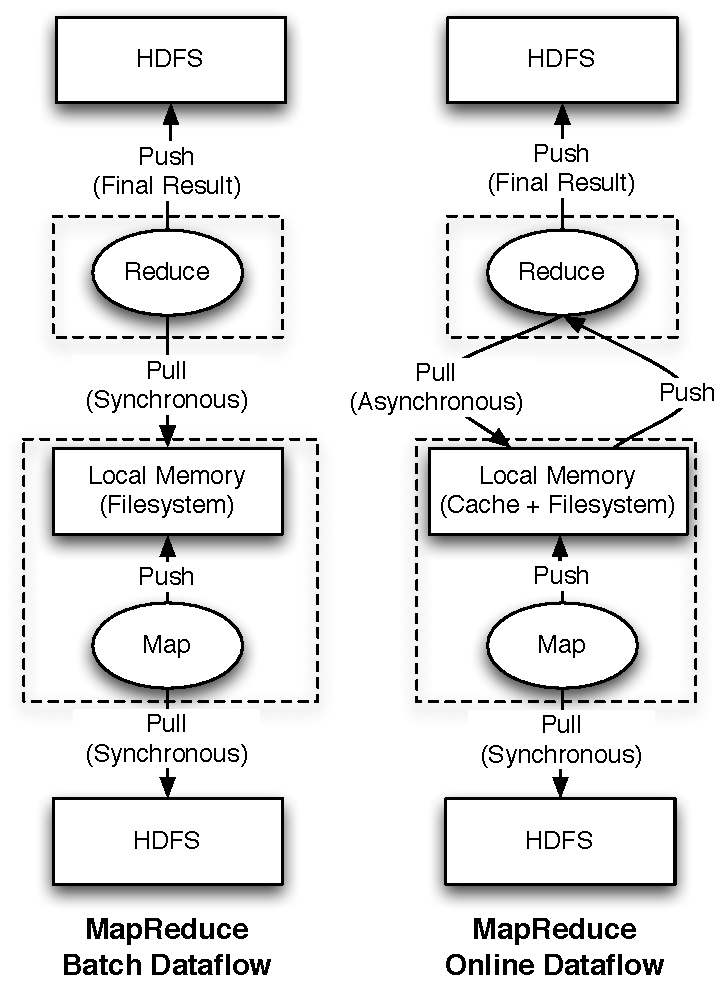
\includegraphics[width=0.90\linewidth]{figures/dataflow_arch.pdf}
%  \caption{Hadoop dataflow for batch (left) and pipelined (right) processing of MapReduce computations.}
%  \label{ch:hop:fig:pipeline}
%\end{figure}
%Figure~\ref{ch:hop:fig:pipeline} depicts the dataflow of two MapReduce
%configurations.  The dataflow on the left describes the materialization
%approach followed by stock Hadoop, while the dataflow on the right allows
%pipelining.  In the remainder of this section, we present our design and
%implementation for the pipelined Hadoop dataflow.  We describe how our design
%supports fault tolerance (Section~\ref{ch:hop:sec:ft}), and discuss the
%interaction between pipelining and task scheduling
%(Section~\ref{ch:hop:sec:pipeline-sched}).

\subsection{Pipelining Within A Job}
\label{ch:hop:sec:intra-pipe}

As described in Chapter~\ref{ch:hadoop:sec:reducetask}, reduce tasks
traditionally issue HTTP requests to {\em pull} their input from each {\TT}
that hosted a map task belonging to the same job.  A \TT is responsible for
serving these HTTP requests, which could occur long after the map task's
execution.  This means that map task execution is completely decoupled from
reduce task execution.  To support pipelining, we modified the \TT serving
component to {\em push} data to reducers as it is produced by the map tasks,
while still maintaining the decoupling of these two steps.  To give an
intuition for how this works, we begin by describing a straightforward
pipelining design, and then discuss the changes we had to make to achieve good
performance.

\subsubsection{Na\"{\i}ve Pipelining}
\label{ch:hop:sec:naive}

We begin with a na\"{\i}ve implementation that sends data directly from map to
reduce tasks via a TCP socket.  Immediately, this design couples the execution
of map and reduce task executions, forcing us to schedule {\em all} reduce
tasks before any one map task.  Consequently, this design does not scale, most
notably when there is not sufficient reduce task slot capacity, but there are
other ramifications that we discuss here before converging on the true HOP
design.

Recall, that when a client submits a new job to Hadoop, the {\JT} assigns the
map and reduce tasks associated with the job to the available {\TT} slots.  For
purposes of {\em this} discussion, we must assume that there are enough free
slots to assign all reduce tasks in a job.  We modified Hadoop so that each
reduce task contacts every map task upon initiation of the job, and opens a TCP
socket which will be used to pipeline the output of the map function.  As each
map output record is produced, the mapper determines which partition (reduce
task) the record should be sent to, and immediately sends it via the
appropriate socket.

A reduce task accepts the pipelined data it receives from each map task and
stores it in an in-memory buffer, spilling sorted runs of the buffer to disk as
needed. Once the reduce task learns that every map task has completed, it
performs a final merge of all the sorted runs and applies the user-defined
reduce function as normal.

\subsubsection{Refinements}
\label{ch:hop:sec:pipe-refine}

While the algorithm described above is straightforward, it suffers from several
practical problems.  First, it is possible that there will not be enough slots
available to schedule every task in a new job.  Opening a socket between every
map and reduce task also requires a large number of TCP connections.  A simple
tweak to the na\"{\i}ve design solves both problems: if a reduce task has not
yet been scheduled, any map tasks that produce records for that partition
simply write them to disk.  When the map task completes, it registers the output
it was not able to send with the host \TT serving component.  Once the reduce
task is assigned a slot, it can then pull the records from the map task's host
\TT, as in regular Hadoop.  To reduce the number of concurrent TCP connections,
each reducer can be configured to pipeline data from a bounded number of
mappers at once; the reducer will pull data from the remaining map tasks in the
traditional Hadoop manner.

Our initial pipelining implementation suffered from a second problem: the map
function was invoked by the same thread that wrote output records to the
pipeline sockets.  This meant that if a network I/O operation blocked (e.g.,
because the reducer was over-utilized), the mapper was prevented from doing
useful work.  Pipeline stalls should not prevent a map task from making
progress -- especially since, once a task has completed, it frees a {\TT} slot
to be used for other purposes.  We solved this problem by running the map
function in a separate thread that stores its output in an in-memory buffer,
and then having another thread periodically send the contents of the buffer to
the connected reducers.~\footnote{This code was based on the existing Hadoop
SpillThread component, which is responsible for writing map output to disk
concurrently with the ``map function.''}

\subsubsection{Granularity of Map Output}
\label{ch:hop:sec:mapout}

Another problem with the na\"{\i}ve design is that it eagerly sends each record
as soon as it is produced, which prevents the use of map-side combiners.
Imagine a job where the reduce key has few distinct values (e.g., gender), and
the reduce applies an algebraic aggregate function (e.g., count).  As discussed
in Chapter~\ref{ch:hadoop:sec:progmodel}, combiners allow map-side
``pre-aggregation'': by applying a reduce-like function to each distinct key at
the mapper, network traffic can often be substantially reduced.  Eagerly
pipelining each record as it is produced prevents the use of these map-side
combiners.

Another related problem is that eager pipelining moves some of the sorting work
from the mapper to the reducer.  Recall from
Chapter~\ref{ch:hadoop:sec:maptask}, that in the blocking architecture, map
tasks generate sorted spill files: all the reduce task must do is merge
together the pre-sorted map output for each partition.  In the na\"{\i}ve
pipelining design, map tasks send output records as they are generated, so a
reducer (scheduled early) must perform a full external sort.  Because the
number of map tasks typically far exceeds the number of
reduces~\cite{mapreduce-osdi}, moving more work to the reducer increased
response time, as shown in our experiments (Chapter~\ref{ch:hop:sec:perf}).

To avoid a heavy reduce task sort, instead of sending the buffer contents to
reducers directly, we wait for the buffer to grow to a threshold size.  The
mapper then (quick) sorts the output by partition and reduce key, applies the
combiner function, and writes the buffer to disk using the Hadoop spill file
format described in Figure~\ref{ch:hadoop:fig:mapoutput}.  Next, we arranged
for the {\TT} serving component at each node to handle pipelining data to
reduce tasks.  Map tasks register spill files with the {\TT} via
RPCs.~\footnote{We extended the existing RPC Hadoop interface to include
information on individual spill files.  Having the spill files be in the same
format allowed us to reuse much of the stock Hadoop serving code i.e., I/O file
formats/streams.}  If the reducers are able to keep up with the production of
map outputs and the network is not a bottleneck, a spill file will be sent to a
reducer soon after it has been produced (in which case, the spill file is
likely still resident in the map machine's kernel buffer cache).  However, if a
reducer begins to fall behind, the number of unsent spill files will grow.

When a map task generates a new spill file, it first queries the {\TT} for the
number of unsent spill files.  If this number grows beyond a certain threshold
(two unsent spill files in our experiments), the map task does not immediately
register the new spill file with the {\TT}.  Instead, the mapper will
accumulate multiple spill files.  Once the queue of unsent spill files falls
below the threshold, the map task merges and combines the accumulated spill
files into a single file, and then resumes registering its output with the
{\TT}.  This simple flow control mechanism has the effect of {\em adaptively}
moving load from the reducer to the mapper or vice versa, depending on which
node is the current bottleneck.

A similar mechanism is also used to control how aggressively the combiner
function is applied.  The map task records the ratio between the input and
output data sizes whenever it invokes the combiner function.  If the combiner
is effective at reducing data volumes, the map task accumulates more spill
files (and applies the combiner function to all of them) before registering
that output with the {\TT} for pipelining.\footnote{Our current prototype uses
a simple heuristic: if the combiner reduces data volume by $\frac{1}{k}$ on
average, we wait until $k$ spill files have accumulated before registering them
with the {\TT}.  A better heuristic would also account for the computational
cost of applying the combiner function.}

The connection between pipelining and adaptive query processing techniques has
been observed elsewhere (e.g.,~\cite{eddies, bamboo}).  The adaptive scheme
outlined above is relatively simple, but we believe that adapting to feedback
along pipelines has the potential to significantly improve the utilization of
MapReduce clusters.

\subsection{Pipelining Between Jobs}
\label{ch:hop:sec:inter-pipe}

Many practical computations cannot be expressed as a single MapReduce job, and
the outputs of higher-level languages like Pig~\cite{pig-sigmod} typically involve
multiple jobs.  In the traditional Hadoop architecture, the output of each job
is written to HDFS in the reduce step and then immediately read back from HDFS
by the map step of the next job. Furthermore, the {\JT} cannot schedule a
consumer job until the producer job has completed, because scheduling a map task
requires knowing the HDFS block locations of the map's input split.

In our modified version of Hadoop, the reduce tasks of one job can optionally
pipeline their output directly to the map tasks of the next job, sidestepping
the need for expensive fault-tolerant storage in HDFS for what amounts to a
temporary file.  Unfortunately, the computation of the reduce function from the
previous job and the map function of the next job cannot be overlapped: the
final result of the reduce step cannot be produced until all map tasks have
completed, which prevents effective pipelining.  However, we describe later how
online aggregation and continuous query pipelines can publish ``snapshot''
outputs that can indeed pipeline between jobs.

\subsection{Fault Tolerance}
\label{ch:hop:sec:ft}

% nrc: (1) Quantify the overhead added by tracking map task origin (2)
% Did we implement the "don't rerun map task from scratch" idea?

Our pipelined Hadoop implementation is robust to the failure of both
map and reduce tasks. To recover from map task failures, we added
bookkeeping to the reduce task to record which map task produced each
pipelined spill file. To simplify fault-tolerance, the reducer treats
the output of a pipelined map task as ``tentative'' until the {\JT}
informs the reducer that the map task has committed successfully. The
reducer can merge together spill files generated by the same
uncommitted mapper, but will not combine those spill files with the
output of other map tasks until it has been notified that the map task
has committed. Thus, if a map task fails, each reduce task can ignore
any tentative spill files produced by the failed map attempt. The
{\JT} will take care of scheduling a new map task attempt, as in stock
Hadoop. 

If a reduce task fails and a new copy of the task is started, the new
reduce instance must be sent all the input data that was sent to the
failed reduce attempt. If map tasks operated in a purely pipelined
fashion and discarded their output after sending it to a reducer, this
would be difficult. Therefore, map tasks retain their output data on
the local disk for the complete job duration. This allows the map's output to be 
reproduced if any reduce tasks fail. For batch jobs, the key advantage of our architecture is
that reducers are not blocked waiting for the complete output of the
task to be written to disk.

Our technique for recovering from map task failure is straightforward, but
places a minor limit on the reducer's ability to merge spill files. To avoid
this, we envision introducing a ``checkpoint'' concept: as a map task runs, it
will periodically notify the {\JT} that it has reached offset $x$ in its input
split. The {\JT} will notify any connected reducers; map task output that was
produced before offset $x$ can then be merged by reducers with other map task
output as normal. To avoid duplicate results, if the map task fails, the new map
task attempt resumes reading its input at offset $x$. This technique would also
reduce the amount of redundant work done after a map task failure or during
speculative execution of ``backup'' tasks~\cite{mapreduce-osdi}.

\subsection{Performance Evaluation}
\label{ch:hop:sec:perf}

A thorough performance comparison between pipelining and blocking is not the
focus of this work.  However, as future work we plan to investigate a
rule-based (e.g., Evita Raced) optimizer for Hadoop MapReduce that considers
pipelined plans in its search strategy.  Here, we demonstrate that pipelining
can reduce job completion times in some configurations and should be considered
by any such optimizer.

We report performance using both large (512MB) and small (32MB) HDFS block
sizes using a single workload (a wordcount job over randomly-generated text).
Since the words were generated using a uniform distribution, map-side combiners
were ineffective for this workload.  We performed all experiments using
relatively small clusters of Amazon EC2 nodes.  We also did not consider
performance in an environment where multiple concurrent jobs are executing
simultaneously.

\subsubsection{Background and Configuration}

Before diving into the performance experiments, it is important to further
describe the division of labor in a HOP job, which is broken into task phases.
A map task consists of two work phases: {\em map} and {\em sort}.  Much of the
work performed during the job happens in the {\em map} phase, where the map
function is applied to each record in the input and subsequently sent to an
output buffer.  Once the entire input has been processed, the map task enters
the {\em sort} phase, where a final merge sort of all intermediate spill files
is performed before registering the final output with the \TT.  The progress
reported by a map task corresponds to the {\em map} phase, which is overlapped
with many in-memory record buffer sorts and subsequent spills to local files.

A reduce task in HOP is divided into three work phases: {\em shuffle}, {\em
reduce}, and {\em commit}.  In the {\em shuffle} phase, reduce tasks receive
their portion of the output from each map.  In HOP, the {\em shuffle} phase
consumes 75\% of the overall reduce task progress while the remaining 25\% is
allocated to the {\em reduce} and {\em commit} phase.~\footnote{The stock
version of Hadoop divides the reduce progress evenly among the three phases.
We deviated from this approach because we wanted to focus more on the progress
during the {\em shuffle} phase.} In the {\em shuffle} phase, reduce tasks
periodically perform a merge sort on the already received map output.  These
intermediate merge sorts decrease the amount of sorting work performed at the
end of the {\em shuffle} phase.  After receiving its portion of data from all
map tasks, the reduce task performs a final merge sort and enters the {\em
reduce} phase.

By pushing work from map tasks to reduce tasks more aggressively, pipelining
can enable better overlapping of map and reduce computation, especially when
the node on which a reduce task is scheduled would otherwise be underutilized.
However, when reduce tasks are already the bottleneck, pipelining offers fewer
performance benefits, and may even hurt performance by placing additional load
on the reduce nodes.

The {\em sort} phase in the map task minimizes the merging work that reduce
tasks must perform at the end of the {\em shuffle} phase.  When pipelining is
enabled, the {\em sort} phase is avoided since map tasks have already sent some
fraction of the spill files to concurrently running reduce tasks.  Therefore,
pipelining increases the merging workload placed on the reducer.  The adaptive
pipelining scheme described in Chapter~\ref{ch:hop:sec:mapout} attempts to
ensure that reduce tasks are not overwhelmed with additional load.

We used two Amazon EC2 clusters depending on the size of the experiment:
``small'' jobs used 10 worker nodes, while ``large'' jobs used 20.  Each node
was an ``extra large'' EC2 instances with 15GB of memory and four virtual
cores, each running at 2.4GHz with a 2GB L2 cache.

\subsubsection{Small Job Results}

\begin{figure*}[t]
\ssp
\begin{minipage}{0.5\linewidth}
  \centering
        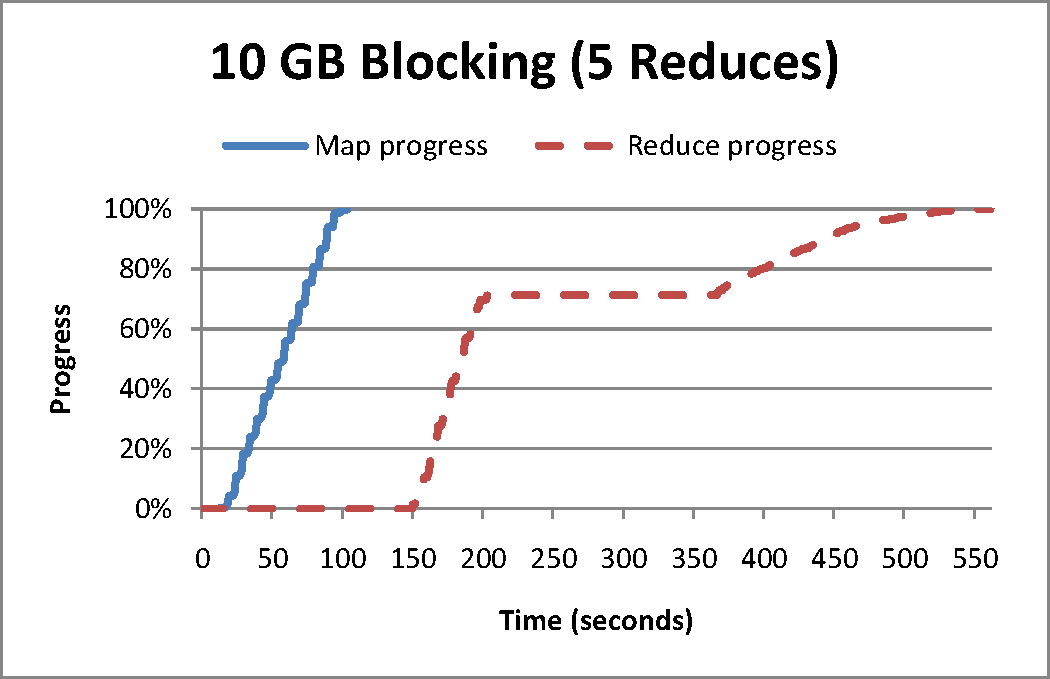
\includegraphics[width=0.90\linewidth]{figures/wc_10gb_20m5r_blocking}
\end{minipage}
\begin{minipage}{0.5\linewidth}
  \centering
        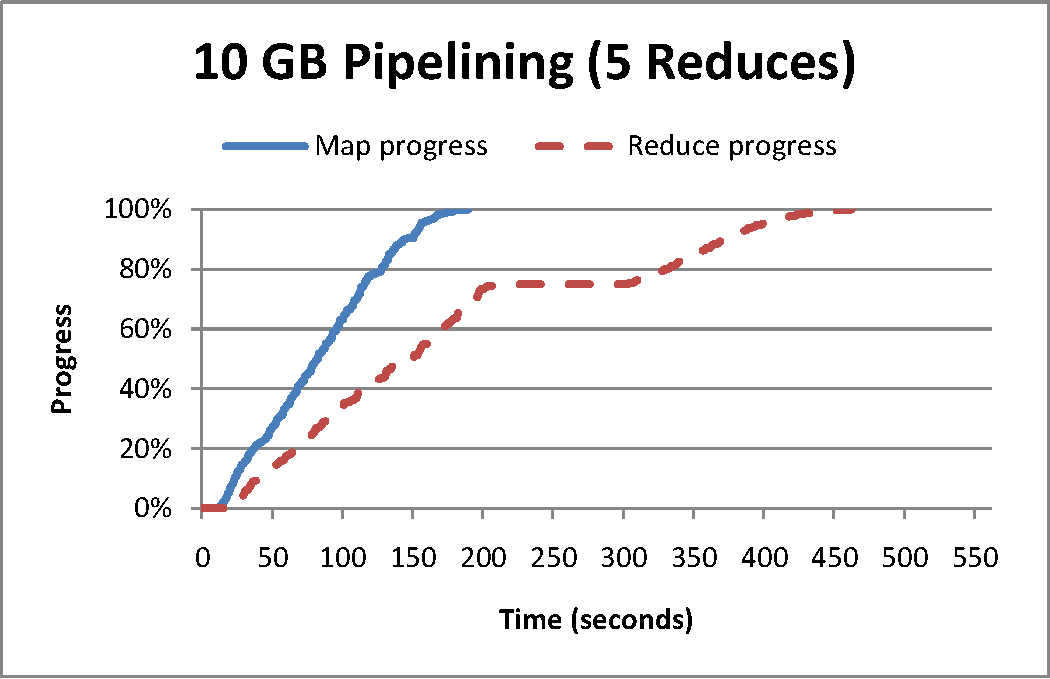
\includegraphics[width=0.90\linewidth]{figures/wc_10gb_20m5r_pipeline}
\end{minipage}
\caption{CDF of map and reduce task completion times for a 10GB wordcount job
  using 20 map tasks and 5 reduce tasks (512MB block size). The total job
  runtimes were 561 seconds for blocking and 462 seconds for pipelining.}
\label{ch:hop:fig:wc1}
\end{figure*}

\begin{figure*}[t]
\ssp
\begin{minipage}{0.5\linewidth}
  \centering
        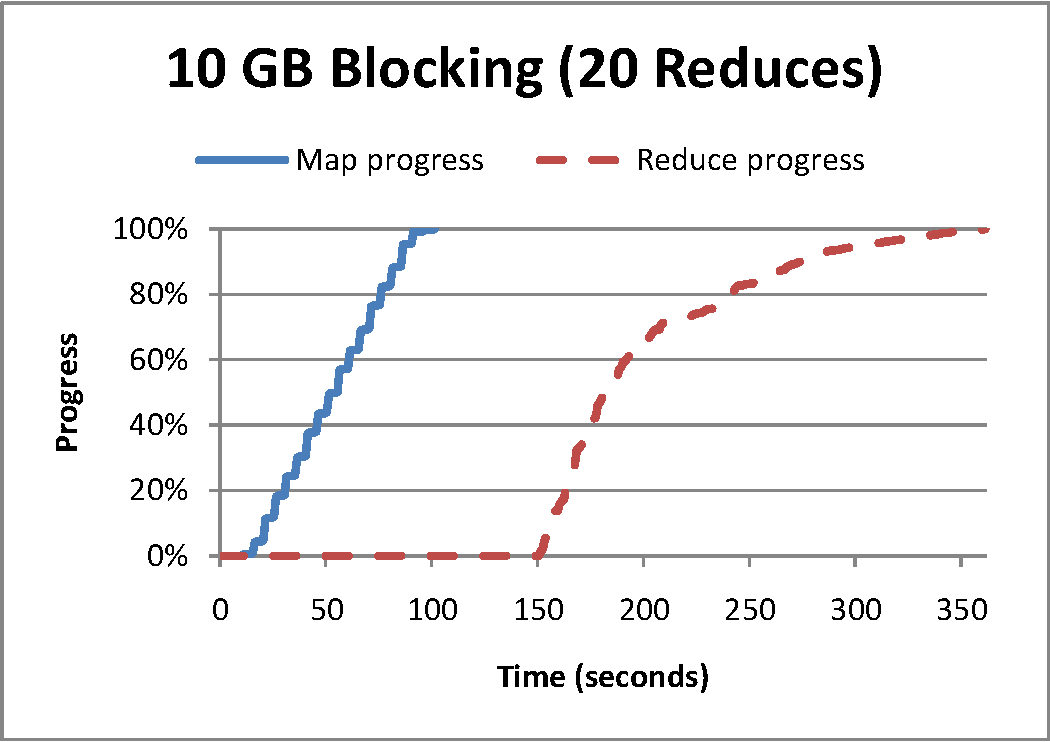
\includegraphics[width=0.88\linewidth]{figures/wc_10gb_20m20r_blocking}
\end{minipage}
\begin{minipage}{0.5\linewidth}
  \centering
        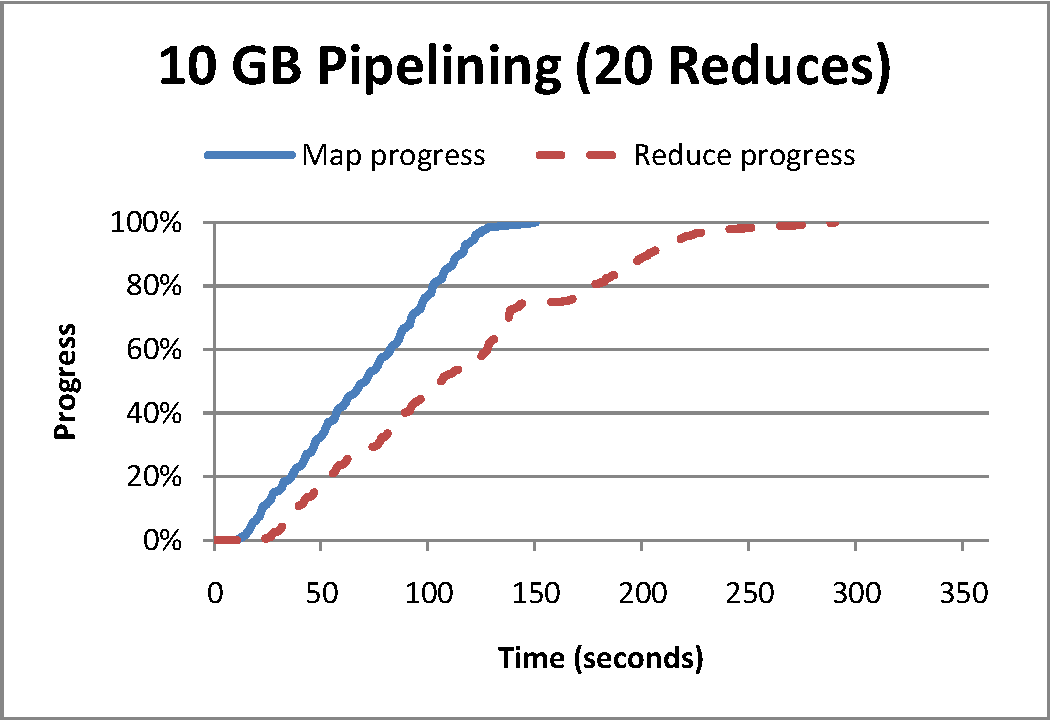
\includegraphics[width=0.90\linewidth]{figures/wc_10gb_20m20r_pipeline}
\end{minipage}
\caption{CDF of map and reduce task completion times for a 10GB wordcount job
  using 20 map tasks and 20 reduce tasks (512MB block size). The total job
  runtimes were 361 seconds for blocking and 290 seconds for pipelining.}
\label{ch:hop:fig:wc2}
\end{figure*}

\begin{figure*}[t]
\ssp
\begin{minipage}{0.5\linewidth}
  \centering
        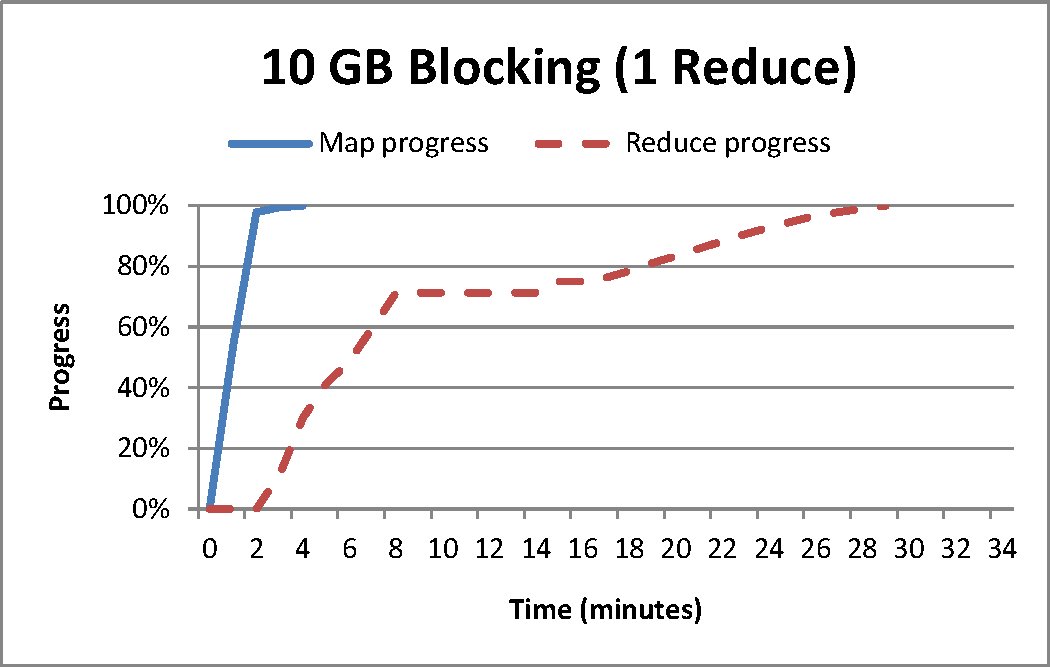
\includegraphics[width=0.95\linewidth]{figures/wc_10gb_20m1r_blocking}
\end{minipage}
\begin{minipage}{0.5\linewidth}
  \centering
        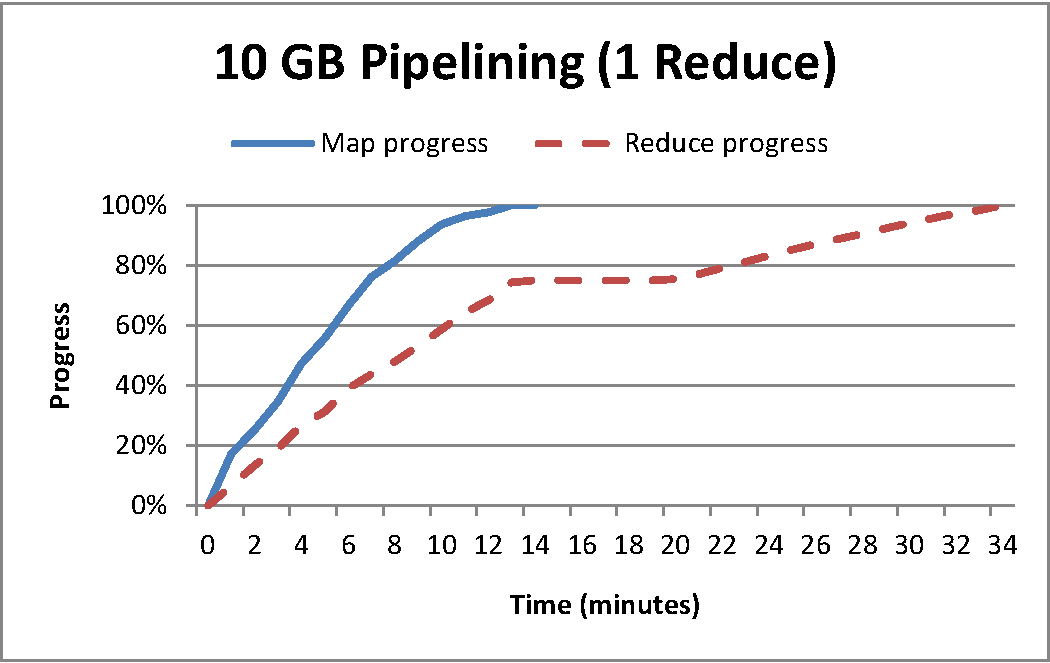
\includegraphics[width=0.95\linewidth]{figures/wc_10gb_20m1r_pipeline}
\end{minipage}
\caption{CDF of map and reduce task completion times for a 10GB wordcount job
  using 20 map tasks and 1 reduce task (512MB block size). The total job
  runtimes were 29 minutes for blocking and 34 minutes for pipelining.}
\label{ch:hop:fig:wc3}
\end{figure*}


Our first experiment focused on the performance of small jobs in an
underutilized cluster.  We ran a 10GB wordcount with a 512MB block size,
yielding 20 map tasks (one per block).  We used 10 worker nodes and configured
each worker to execute at most two map and two reduce tasks simultaneously.  We
ran several experiments to compare the performance of blocking and pipelining
using different numbers of reduce tasks.  For each experiment, we report the
average progress over five separate runs. 

Figure~\ref{ch:hop:fig:wc1} reports the results of a job configured with five
reduce tasks.  A plateau can be seen at 75\% progress for both blocking and
pipelining.  At this point in the job, all reduce tasks have completed the {\em
shuffle} phase; the plateau is caused by the time taken to perform a final
merge of all map output before entering the {\em reduce} phase.  Notice that
the plateau for the pipelining case is shorter.  With pipelining, reduce tasks
receive map outputs much earlier and can begin sorting earlier, thereby
reducing the time required for the final merge.

Figure~\ref{ch:hop:fig:wc2} reports the results with twenty reduce tasks.
Using more reduce tasks decreases the amount of merging that any one reduce
task must perform, which reduces the duration of the plateau at 75\% progress.
In the blocking case, the plateau is practically gone.  However, with
pipelining we still see a small plateau at 75\% that, through further analysis
using \ol{iostat}, can be attributed to extra disk I/Os in the pipelining case.
This extra memory pressure is due to diminished effectiveness of the combiner
in the pipelining case.  Although the response time of pipelining job is better
than the blocking, a job that contains a more effective combiner may be better
executed in blocking mode.

We further note that in both experiments, the map phase finishes faster with
blocking than with pipelining.  This is because pipelining allows reduce tasks
to begin executing earlier and perform more work (sorting and combining);
hence, the reduce tasks compete for resources with the map tasks, causing the
map phase to take slightly longer.  In this case, the increase in map duration
is outweighed by the increase in cluster utilization, resulting in shorter job
completion times: pipelining reduced completion time by 17.7\% with 5 reducers
and by 19.7\% with 20 reducers.

Figure~\ref{ch:hop:fig:wc3} describes an experiment in which we ran a 10GB
wordcount job using a single reduce task.  This caused job completion times to
increase dramatically for both pipelining and blocking, because of the extreme
load placed on the reduce node.  Pipelining delayed job completion by about
17\%, which suggests that our simple adaptive flow control scheme
(Chapter~\ref{ch:hop:sec:mapout}) was unable to move load back to the map tasks
aggressively enough in this (extremely) unbalanced job configuration.

\subsubsection{Large Job Results}

\begin{figure*}[t]
\ssp
\begin{minipage}{0.5\linewidth}
  \centering
        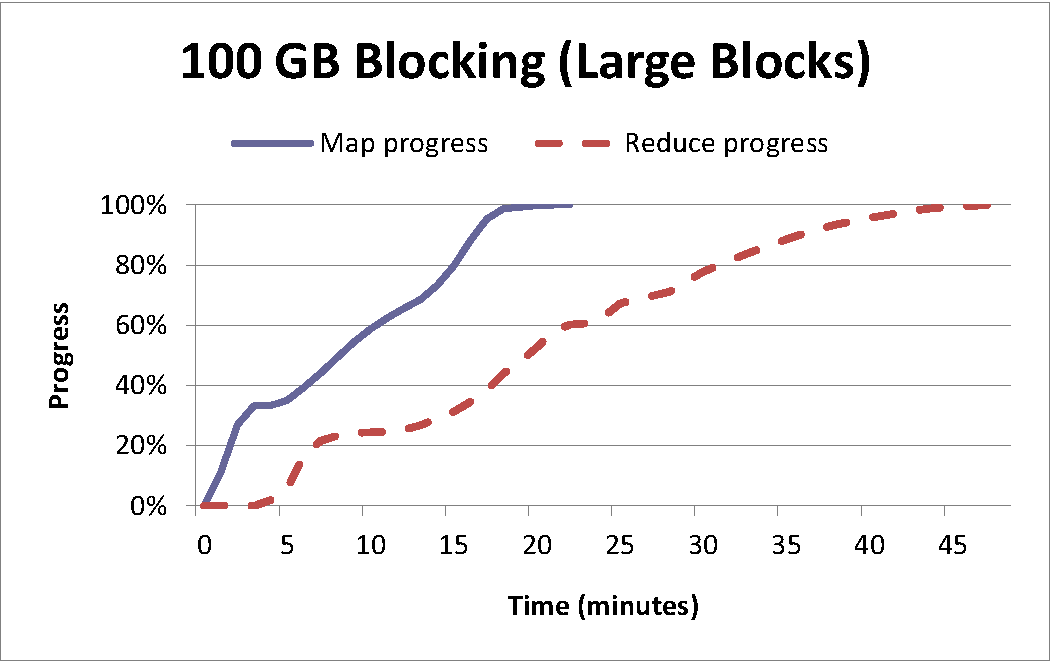
\includegraphics[width=0.95\linewidth]{figures/wc_100gb_240m60r_blocking}
\end{minipage}
\begin{minipage}{0.5\linewidth}
  \centering
        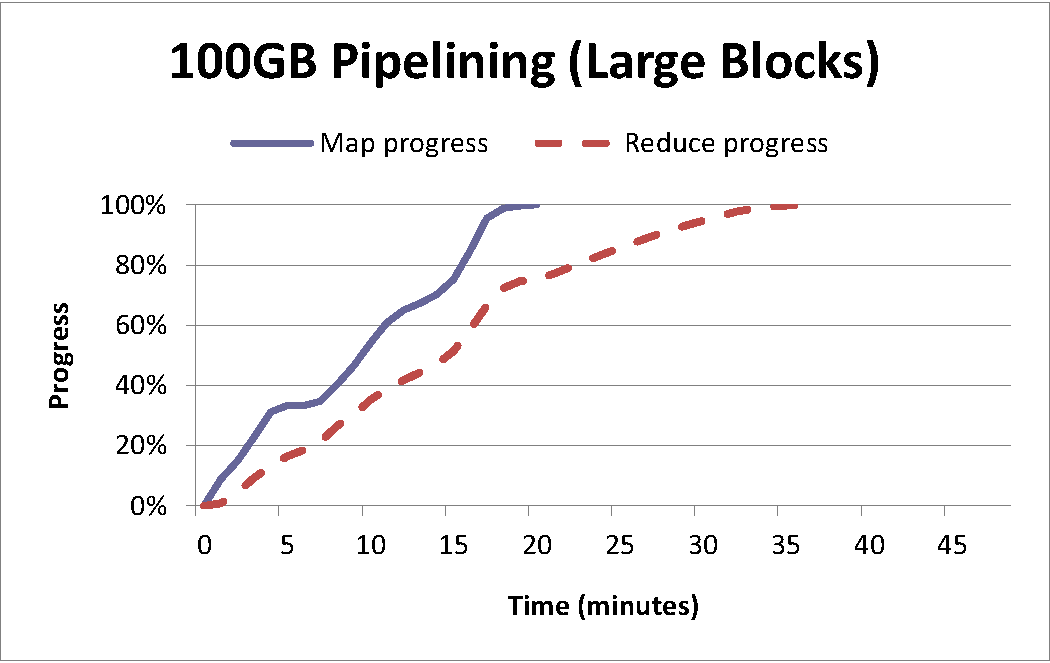
\includegraphics[width=0.95\linewidth]{figures/wc_100gb_240m60r_pipeline}
\end{minipage}
\caption{CDF of map and reduce task completion times for a 100GB wordcount job
  using 240 map tasks and 60 reduce tasks (512MB block size). The total job
  runtimes were 48 minutes for blocking and 36 minutes for pipelining.}
\label{ch:hop:fig:wc4}
\end{figure*}

\begin{figure*}[t]
\ssp
\begin{minipage}{0.5\linewidth}
  \centering
        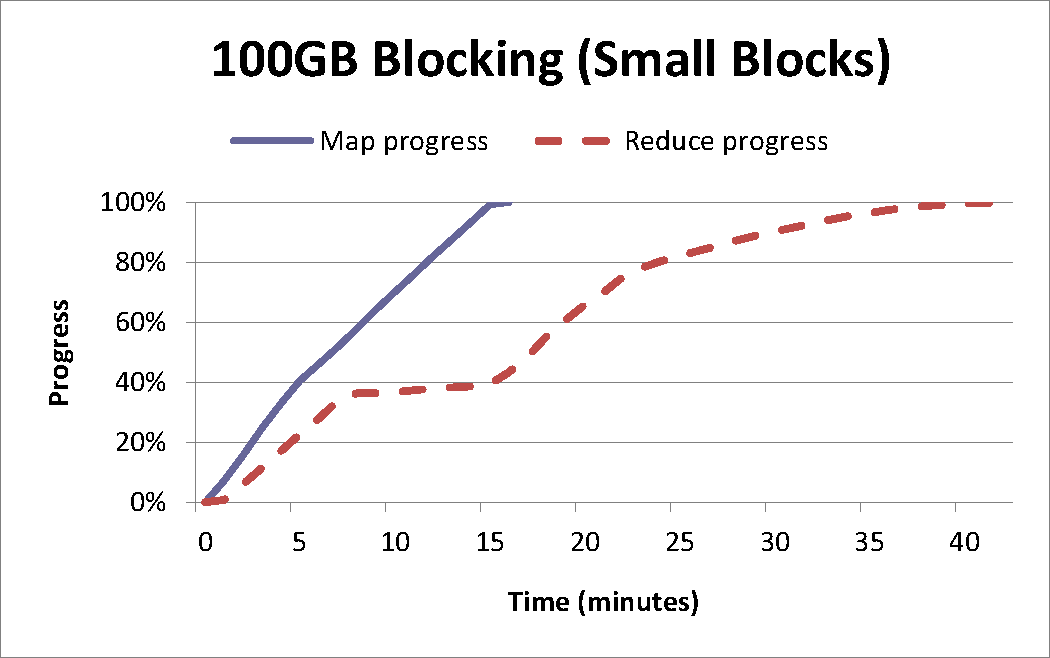
\includegraphics[width=0.95\linewidth]{figures/wc_100gb_3120m60r_blocking}
\end{minipage}
\begin{minipage}{0.5\linewidth}
  \centering
        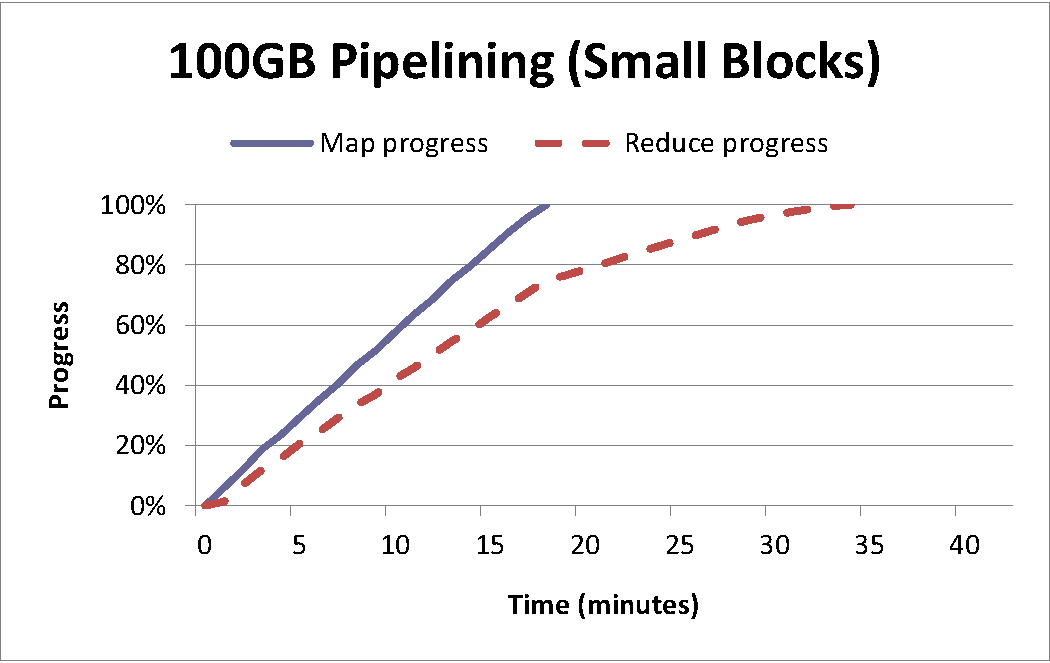
\includegraphics[width=0.95\linewidth]{figures/wc_100gb_3120m60r_pipeline}
\end{minipage}
\caption{CDF of map and reduce task completion times for a 100GB wordcount job
  using 3120 map tasks and 60 reduce tasks (32MB block size). The total job
  runtimes were 42 minutes for blocking and 34 minutes for pipelining.}
\label{ch:hop:fig:wc5}
\end{figure*}

Our second set of experiments focused on the performance of somewhat larger
jobs. We increased the input size to 100GB (from 10GB) and the number of worker
nodes to 20 (from 10). Each worker was configured to execute at most four map
and three reduce tasks, which meant that at most 80 map and 60 reduce tasks
could execute at once. We conducted two sets of experimental runs, each run
comparing blocking to pipelining using either large (512MB) or small (32MB)
block sizes. We were interested in blocking performance with small block sizes
because blocking can effectively emulate pipelining if the block size is small
enough.

Figure~\ref{ch:hop:fig:wc4} reports the performance of a 100GB wordcount job
with 512MB blocks, which resulted in 240 map tasks, scheduled in three waves of
80 tasks each.  The 60 reduce tasks were co-scheduled with the first wave of map
tasks.  In the blocking case, the reduce tasks began working as soon as they
received the output of the first wave, which is why the reduce progress begins
to climb around four minutes (well before the completion of all maps).
Pipelining was able to achieve significantly better cluster utilization, and
hence reduced job completion time by about 25\%.

Comparing the reduce progress in blocking to pipelining, we see that reduce
tasks make more progress during the {\em shuffle} phase when pipelining is
enabled. What is even more interesting is that the {\em reduce} phase is also
shorter in the case of pipelining. The reason for this is subtle; all reduce
tasks enter the {\em phase} around the same time since data is shipped in
smaller increments. In the blocking case, when the final wave of map tasks
finish they all try to send the entire output to reduce tasks at the same time,
which increases the variance on receiving the complete output from all map
tasks. That is, some reduce tasks enter the {\em reduce} phase well in advance
of others.

Figure~\ref{ch:hop:fig:wc5} reports the performance of blocking and pipelining
using 32MB blocks.  While the performance of pipelining remained similar, the
performance of blocking improved considerably, but still trailed somewhat
behind pipelining.  Using block sizes smaller than 32MB did not yield a
significant performance improvement in our experiments.

% \subsection{Discussion}

% As mentioned before, a complete performance evaluation is beyond the scope
% for this paper and we leave such a study for future work.  The focus here was
% to provide some initial insight into the performance benefits of pipelining.
% We also wanted to evaluate the adaptive policy of our pipelining scheme.  To
% this end, we found such a policy paramount in discovering the right amount of
% pipelining to perform based on runtime factors; network capacity and reduce
% task (consumer) load.

%\begin{figure*}[t]
%\begin{minipage}{0.5\linewidth}
%        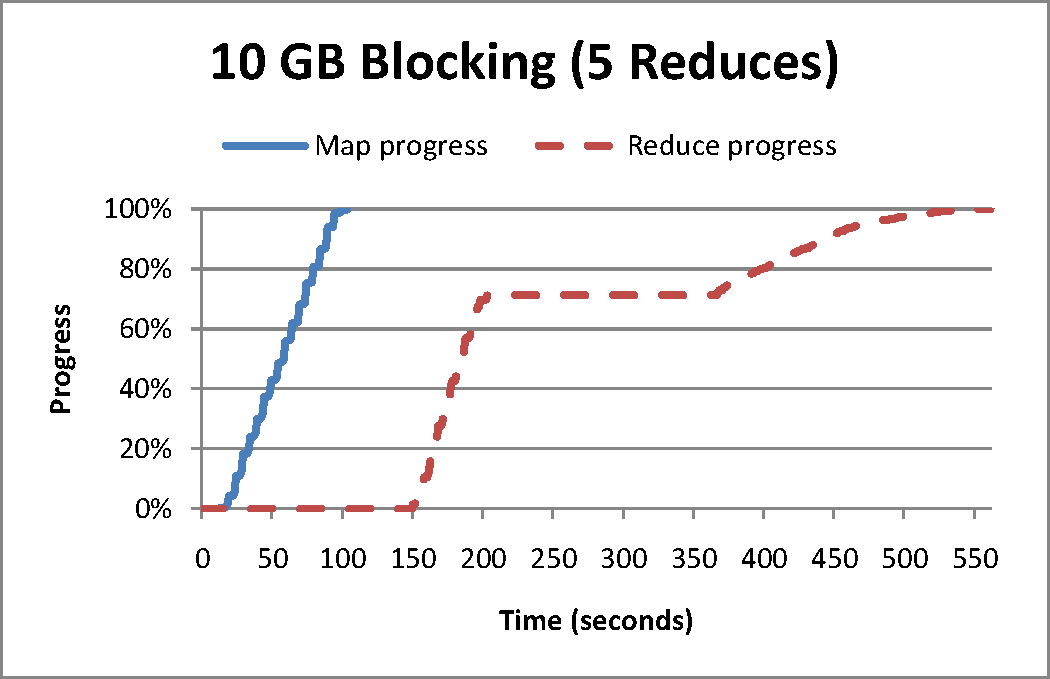
\includegraphics[width=0.95\linewidth]{figures/wc_10gb_20m5r_blocking}
%\end{minipage}
%\begin{minipage}{0.5\linewidth}
%        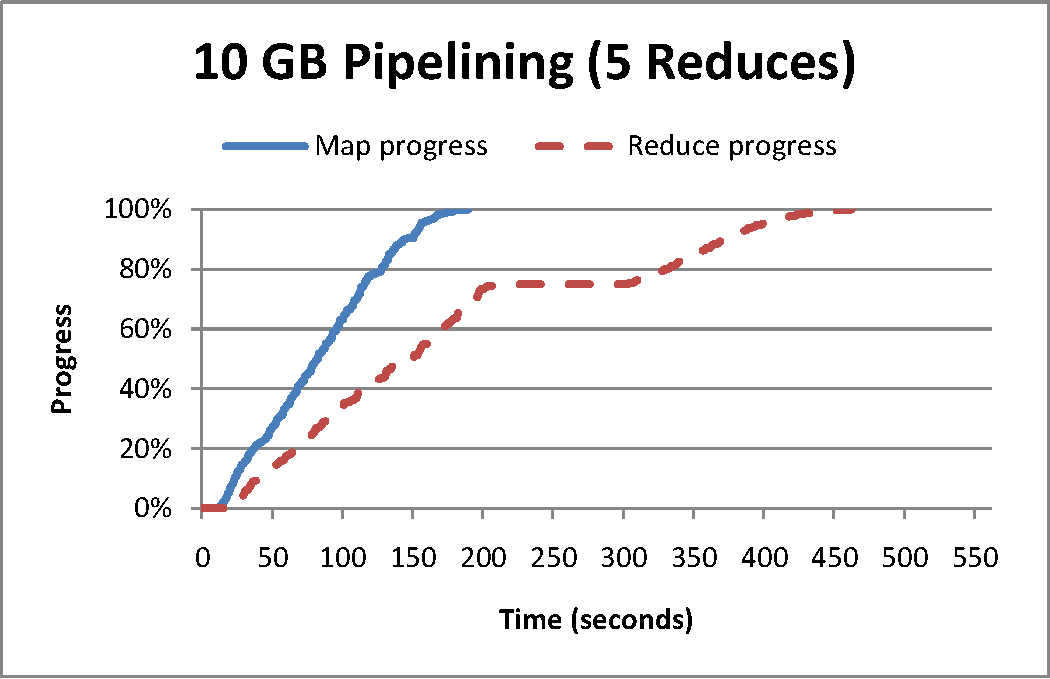
\includegraphics[width=0.95\linewidth]{figures/wc_10gb_20m5r_pipeline}
%\end{minipage}
%\caption{CDF of map and reduce task completion times for a sort job on
%  5.5GB of text extracted from Wikipedia. The total job runtimes were
%  927 seconds for blocking, and 610 seconds for pipelining.}
%\label{fig:sort}
%\end{figure*}

%We conducted a series of performance experiments using a 60-node
%cluster on Amazon EC2. One node executed the Hadoop \JT\ and the HDFS
%\NN, while the remaining 59 nodes served as slaves for running the
%{\TT}s and HDFS {\DN}s. All nodes executed on ``high-CPU medium'' EC2
%instances with 1.7GB of memory and two virtual cores. Each virtual
%core is the equivalent of a 2007-era 2.5Ghz Intel Xeon processor.

%We began by measuring the performance of a simple MapReduce job that
%does not use a combiner. Sorting is commonly used as a benchmark for
%basic MapReduce performance, because of the implicit sort done by the
%reduce phase. We sorted 5.5GB of article text extracted from
%Wikipedia; each word from the text was parsed as a separate
%record. Figure~\ref{fig:sort} describes sort performance on the EC2
%cluster using an HDFS block size of 128MB (yielding 40 map tasks). We
%configured the system to use 59 reducers. In each graph, we give the
%CDF of map and reduce task completion. The left and right graphs
%depict blocking and pipelined performance, respectively.

%Pipelining dominates blocking for this configuration, in part because
%it achieves better cluster utilization: the reduce tasks in the
%blocking job were idle for the first $192$ seconds of the experiment,
%whereas for the pipelined job, reducers began doing useful work within
%$20$ seconds. Note that in a highly-utilized cluster, increased
%pipeline parallelism would not necessarily lead to an improvement in
%total throughput. However, these results suggest that pipelining can
%substantially reduce the response time of an individual job, which can
%often be important (e.g., quickly executing high-priority jobs).


\section{Online Aggregation}
\label{ch:hop:sec:online}

Although MapReduce was originally designed as a batch-oriented system,
it is often used for interactive data analysis: a user submits a job
to extract information from a data set, and then waits to view the
results before proceeding with the next step in the data analysis
process. This trend has accelerated with the development of high-level
query languages that are executed as MapReduce jobs, such as
Hive~\cite{hive-vldb}, Jaql~\cite{jaql}, Pig~\cite{pig-sigmod}, and Sawzall~\cite{sawzall}.

Traditional MapReduce implementations provide a poor interface for interactive
data analysis, because they do not emit any output until the job has been
executed to completion.  In many cases, an interactive user would prefer a
``quick and dirty'' approximation over a correct answer that takes much longer
to compute.  In the database literature, online aggregation has been proposed
to address this problem~\cite{onlineagg}, but the batch-oriented nature of
traditional MapReduce implementations makes these techniques difficult to
apply.  Here, we show how we extended our pipelined Hadoop implementation to
support online aggregation within a single job
(Chapter~\ref{ch:hop:sec:online-single}) and between multiple jobs
(Chapter~\ref{ch:hop:sec:online-multi}).  In
Chapter~\ref{ch:hop:sec:online-eval}, we evaluate online aggregation on two
different data sets, and show that it can yield an accurate approximate answer
long before the job has finished executing.

\subsection{Single-Job Online Aggregation}
\label{ch:hop:sec:online-single}

In HOP, the data records produced by map tasks are sent to reduce tasks shortly
after each record is generated. However, to produce the final output of the job,
the reduce function cannot be invoked until the entire output of every map task
has been produced. We can support online aggregation by simply applying the
reduce function to the data that a reduce task has received so far. We call the
output of such an intermediate reduce operation a {\em snapshot}.

Users would like to know how accurate a snapshot is: that is, how closely a
snapshot resembles the final output of the job.  Accuracy estimation is a hard
problem even for simple SQL queries~\cite{dbo}, and particularly hard for jobs
where the map and reduce functions are opaque user-defined code.  Hence, we
report job {\em progress}, not accuracy: we leave it to the user (or their
MapReduce code) to correlate progress to a formal notion of accuracy.  We
define a simple progress metric later in this chapter.

Snapshots are computed periodically, as new data arrives at each reducer. The
user specifies how often snapshots should be computed, using the progress metric
as the unit of measure. For example, a user can request that a snapshot be
computed when 25\%, 50\%, and 75\% of the input has been seen. The user may also
specify whether to include data from tentative (unfinished) map tasks. This
option does not affect the fault-tolerance design described in
Chapter~\ref{ch:hop:sec:ft}. In the current prototype, each snapshot is stored in a
directory on HDFS\@. The name of the directory includes the progress value
associated with the snapshot. Each reduce task runs independently, and at a
different rate. Once a reduce task has made sufficient progress, it writes a
snapshot to a temporary directory on HDFS, and then atomically renames it to the
appropriate location.

Applications can consume snapshots by polling HDFS in a predictable
location. An application knows that a given snapshot has been
completed when every reduce task has written a file to the snapshot
directory.  Atomic rename is used to avoid applications mistakenly
reading incomplete snapshot files.

Note that if there are not enough free slots to allow all the reduce tasks in a
job to be scheduled, snapshots will not be available for reduce tasks that are
still waiting to be executed. The user can detect this situation (e.g.,\ by
checking for the expected number of files in the HDFS snapshot directory), so
there is no risk of incorrect data, but the usefulness of online aggregation
will be reduced. In the current prototype, we manually configured the cluster to
avoid this scenario. The system could also be enhanced to avoid this pitfall
entirely by optionally waiting to execute an online aggregation job until there
are enough reduce slots available.

\subsubsection{Progress Metric}
\label{ch:hop:sec:online-metric}

Hadoop provides support for monitoring the progress of task executions.  As
each map task executes, it is assigned a {\em progress score} in the range
[0,1], based on how much of its input the map task has consumed.  We reused
this feature to determine how much progress is represented by the current input
to a reduce task, and hence to decide when a new snapshot should be taken.
When the transfer of a spill file to a reduce task occurs, we include a small
amount of meta-data that indicates the map's current progress score, relative
to that spill file.  To compute the overall progress score for a reduce step
snapshot, we take the average of the progress scores associated with each map's
data residing on the reduce task prior to executing the snapshot. 

Note that it is possible to have a map task that has not pipelined {\em any}
output to a reduce task, either because the map task has not been scheduled yet
(there are no free {\TT} slots), the map tasks does not produce any output for
the given reduce task, or because the reduce task has been configured to only
pipeline data from at most $k$ map tasks concurrently.  To account for this, we
need to scale the progress metric to reflect the portion of the map tasks that
a reduce task has pipelined data from: if a reducer is connected to
$\frac{1}{n}$ of the total number of map tasks in the job, we divide the
average progress score by $n$.

This progress metric could easily be made more sophisticated: for example, an
improved metric might include the selectivity ($|output|/|input|$) of each map task, the
statistical distribution of the map task's output, and the effectiveness of each
map task's combine function, if any. 
% We also assume that each map task
% constitutes a random sample from the input file; otherwise, the scale
% factor we use to account for unavailable map input will introduce
% bias. 
Although we have found our simple progress metric to be
sufficient for most experiments we describe below, this clearly
represents an opportunity for future work.

\subsection{Multi-Job Online Aggregation}
\label{ch:hop:sec:online-multi}

Online aggregation is particularly useful when applied to a long-running
analysis task composed of multiple MapReduce jobs.  As described in
Chapter~\ref{ch:hop:sec:inter-pipe}, our version of Hadoop allows the output of
a reduce task to be sent directly to map tasks.  This feature can be used to
support online aggregation for a sequence of jobs.

Suppose that $j_1$ and $j_2$ are two MapReduce jobs, and $j_2$ consumes the
output of $j_1$.  When $j_1$'s reducers compute a snapshot to perform online
aggregation, that snapshot is written to HDFS, and also sent directly to the
map tasks of $j_2$.  The map and reduce steps for $j_2$ are then computed as
normal, to produce a snapshot of $j_2$'s output.  This process can then be
continued to support online aggregation for an arbitrarily long sequence of
jobs.
  
Unfortunately, inter-job online aggregation has some drawbacks.  First, the
output of a reduce function is not ``monotonic'': the output of a reduce
function on the first 50\% of the input data may not be obviously related to
the output of the reduce function on the first 25\%.  Thus, as new snapshots
are produced by $j_1$, $j_2$ must be recomputed from scratch using the new
snapshot.  As with inter-job pipelining (Chapter~\ref{ch:hop:sec:inter-pipe}),
this could be optimized for reduce functions that are declared to be
distributive or algebraic aggregates~\cite{datacube}.

To support fault-tolerance for multi-job online aggregation, we consider three
cases. Tasks that fail in $j_1$ recover as described in Chapter~\ref{ch:hop:sec:ft}.
If a task in $j_2$ fails, the system simply restarts the failed task. Since
subsequent snapshots produced by $j_1$ are taken from a superset of the mapper
output in $j_1$, the next snapshot received by the restarted reduce task in
$j_2$ will have a higher progress score. To handle failures in $j_1$, tasks in
$j_2$ cache the most recent snapshot received by $j_1$, and replace it when they
receive a new snapshot with a higher progress metric. If tasks from both jobs
fail, a new task in $j_2$ recovers the most recent snapshot from $j_1$ that was
stored in HDFS and then wait for snapshots with a higher progress score.

%Figure~\ref{fig:snapshot} depicts an inter-job dataflow for batch
%mode (left) and a dataflow that supports online aggregation
%(right). The batch mode forces jobs to read the final output of other
%jobs from HDFS\@.  

%%We support not only reading snapshots from HDFS but
%%also pipelining snapshots directly to jobs that request them. 
% In addition to reading snapshots from HDFS, we support pipelining
% snapshots directly to the jobs that request them.
% This is
% supported via an asynchronous request call interface exported by
% each reduce task, through which map tasks from other jobs can request
% snapshots and even the final output. The final output is concurrently
% written to HDFS for fault tolerance, unless otherwise specified in the
% configuration of the job.
  
% nrc: Discuss progress metric for inter-job OA
  
\subsection{Evaluation}
\label{ch:hop:sec:online-eval}

\begin{figure}
\ssp
  \centering
    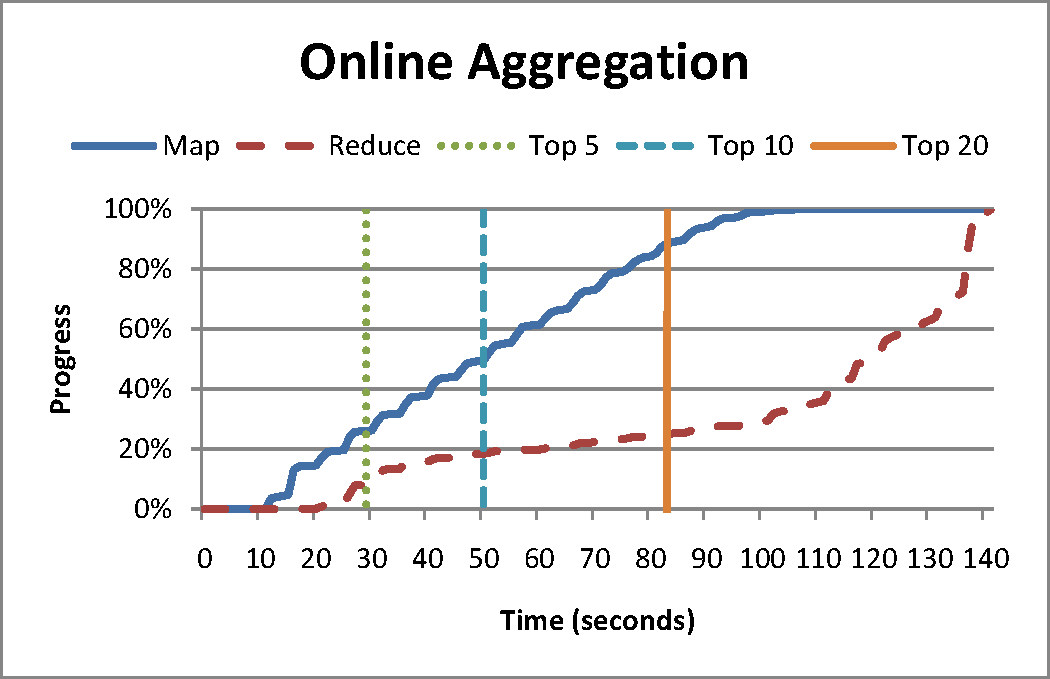
\includegraphics[width=0.7\linewidth]{figures/top100_online_wiki}
    \caption{Top-100 query over 5.5GB of Wikipedia article text. The vertical
      lines describe the increasing accuracy of the approximate answers produced
      by online aggregation.}
\label{fig:topkonlinewiki}
\vspace{-10pt}
\end{figure}

To evaluate the effectiveness of online aggregation, we performed two
experiments on Amazon EC2 using different data sets and query workloads.  In
our first experiment, we wrote a ``Top-$K$'' query using two MapReduce jobs:
the first job counts the frequency of each word and the second job selects the
$K$ most frequent words.  We ran this workload on 5.5GB of Wikipedia article
text stored in HDFS, using a 128MB block size.  We used a 60-node EC2 cluster;
each node was a ``high-CPU medium'' EC2 instance with 1.7GB of RAM and 2
virtual cores.  A virtual core is the equivalent of a 2007-era 2.5Ghz Intel
Xeon processor.  A single EC2 node executed the Hadoop \JT\ and the HDFS \NN,
while the remaining nodes served as slaves for running the {\TT}s and HDFS
{\DN}s.

% To evaluate inter-job dataflow with online aggregation we wrote a
% Top-$K$ query using two MapReduce jobs and executed it on 5.5GB of
% Wikipedia article text. The first job performs a wordcount on the
% words contained in each article.  A reducer from the first job will
% output a list of the Top-$K$ words observed in its partition. The key
% in this output is the word, and the value is the word count. Each map
% task in the subsequent job is assigned to an output from a single
% reduce task. The map function reverses the key-value order, and sends
% that result (sorted by count in descending order) to a single reduce
% task.  The single reduce task merges the sorted lists from each mapper
% and returns the first $K$ words.

% nrc: What does this experiment have to do with online aggregation?
% Figure~\ref{fig:topkwiki} reports the result of a Top-100 query over
% 5.5GB of Wikipedia article text. The left graph represents the
% blocking case as indicated by the idle period in the progress of the
% reduce tasks. The first map tasks finish around 100 seconds into the
% job, which is where the reduce tasks begin to make progress. The
% right graph shows a more balanced load. The reduce tasks
% being receiving mapper output almost immediately following the job
% execution, contributing to the early completion time of the job.

Figure~\ref{fig:topkonlinewiki} shows the results of inter-job online
aggregation for a Top-100 query.  Our accuracy metric for this experiment is
post-hoc --- we note the time at which the Top-$K$ words in the snapshot are
the Top-$K$ words in the final result.  Although the final result for this job
did not appear until nearly the end, we did observe the Top-5, 10, and 20
values at the times indicated in the graph.  The Wikipedia data set was biased
toward these Top-K words (e.g., ``the'', ``is'', etc.), which remained in their
correct position throughout the lifetime of the job.

\subsubsection{Approximation Metrics}

\begin{figure*}[ht]
\ssp
  \centering
  \subfloat[][Relative approximation error over time]{\label{fig:approx-relative}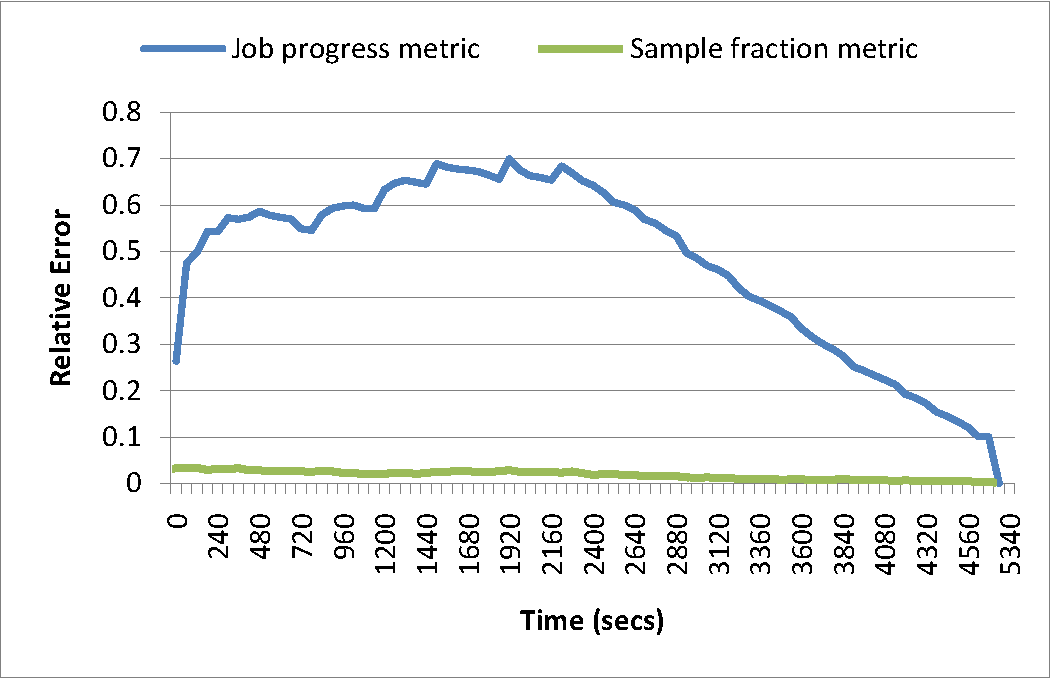
\includegraphics[width=0.48\linewidth]{figures/aprx-click-hour.pdf}}
  \subfloat[][Example approximate answer]{\label{fig:approx-hour}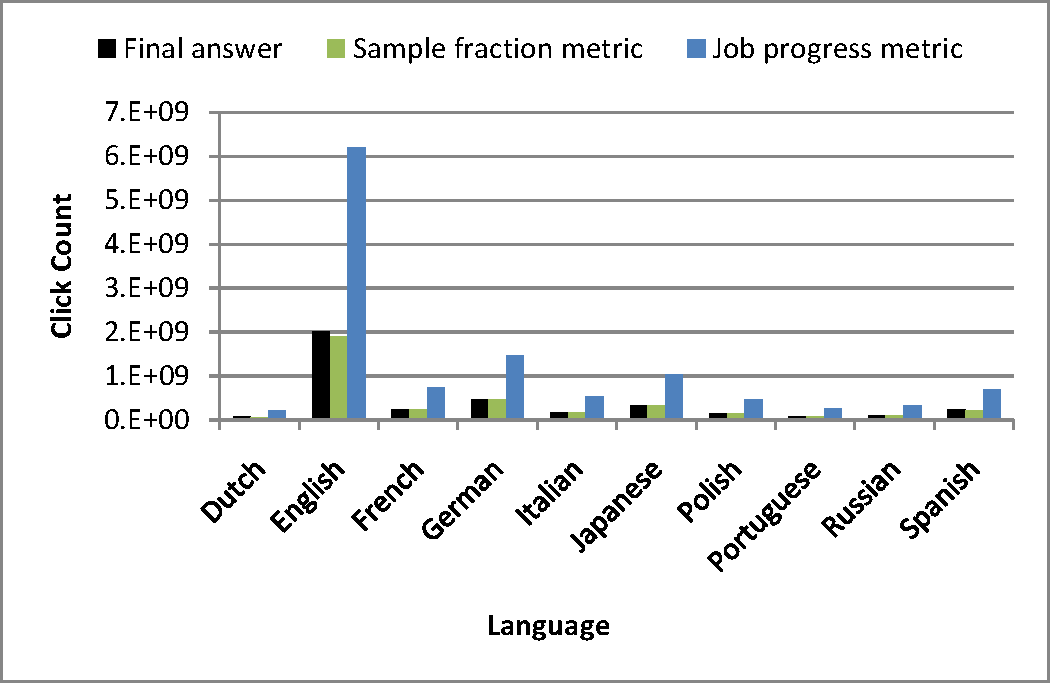
\includegraphics[width=0.48\linewidth]{figures/aprx-click-hour-actual.pdf}}
  \caption{Comparison of two approximation
    metrics. Figure~\protect\subref{fig:approx-relative} shows the relative error for
    each approximation metric over the runtime of the job, averaged over all
    groups. Figure~\protect\subref{fig:approx-hour} compares an example approximate
    answer produced by each metric with the final answer, for each language and for a single hour.}
\label{fig:approx}
\end{figure*}

In our second experiment, we considered the effectiveness of the job progress
metric described in Chapter~\ref{ch:hop:sec:online-metric}. Unsurprisingly, this metric
can be inaccurate when it is used to estimate the accuracy of the approximate
answers produced by online aggregation. In this experiment, we compared the job
progress metric with a simple user-defined metric that leverages knowledge of
the query and data set. HOP allows such metrics, although developing such a
custom metric imposes more burden on the programmer than using the generic
progress-based metric.

We used a data set containing seven months of hourly page view statistics for
more than 2.5 million Wikipedia articles~\cite{wikistats}. This constituted
320GB of compressed data (1TB uncompressed), divided into 5066 compressed
files. We stored the data set on HDFS and assigned a single map task to each
file, which was decompressed before the map function was applied.

We wrote a MapReduce job to count the total number of page views for each
language and each hour of the day. In other words, our query grouped by language
and hour of day, and summed the number of page views that occurred in each
group. To enable more accurate approximate answers, we modified the map function
to include the fraction of a given hour that each record represents. The reduce
function summed these fractions for a given hour, which equated to one for all
records from a single map task. Since the total number of hours was known ahead
of time, we could use the result of this sum over all map outputs to determine
the total fraction of each hour that had been sampled. We call this user-defined
metric the ``sample fraction.''

To compute approximate answers, each intermediate result was scaled up using two
different metrics: the generic metric based on job progress and the sample
fraction described above. Figure~\ref{fig:approx-relative} reports the relative
error of the two metrics, averaged over all groups. Figure~\ref{fig:approx-hour}
shows an example approximate answer for a single hour using both metrics
(computed two minutes into the job runtime). This figure also contains the final
answer for comparison. Both results indicate that the sample fraction metric provides a
much more accurate approximate answer for this query than the progress-based
metric.

Job progress is clearly the wrong metric to use for approximating the final
answer of this query. The primary reason is that it is too coarse of a
metric. Each intermediate result was computed from some fraction of each
hour. However, the job progress assumes that this fraction is uniform across all
hours, when in fact we could have received much more of one hour and much less
of another. This assumption of uniformity in the job progress resulted in a
significant approximation error. By contrast, the sample fraction scales the
approximate answer for each group according to the actual fraction of data seen for
that group, yielding much more accurate approximations.

\section{Continuous Queries}
\label{ch:hop:sec:continuous}

MapReduce is often used to analyze streams of constantly-arriving
data, such as URL access logs~\cite{mapreduce-osdi} and system console
logs~\cite{sosp-mining}. Because of traditional constraints on MapReduce, this 
is done in large batches that can only provide periodic views of activity.
This introduces
significant latency into a data analysis process that ideally should run in 
near-real time. It is also
potentially inefficient: each new MapReduce job does not have access
to the computational state of the last analysis run, so this state
must be recomputed from scratch. The programmer can manually save the
state of each job and then reload it for the next analysis operation,
but this is labor-intensive.

Our pipelined version of Hadoop allows an alternative architecture:
MapReduce jobs that run {\em continuously}, accepting new data as it
becomes available and analyzing it immediately. This allows for near-real-time
analysis of data streams, and thus
allows the MapReduce programming model to be applied to domains such
as environment monitoring and real-time fraud detection.

In this section, we describe how HOP supports continuous MapReduce
jobs, and how we used this feature to implement a rudimentary
cluster monitoring tool.

\subsection{Continuous MapReduce Jobs}
A bare-bones implementation of continuous MapReduce jobs is easy to
implement using pipelining. No changes are needed to implement
continuous map tasks: map output is already delivered to the
appropriate reduce task shortly after it is generated. We added an
optional ``flush'' API that allows map functions to force their current
output to reduce tasks. When a reduce task is unable to accept such data, the mapper framework
stores it locally and sends it at a later time. 
With proper scheduling of reducers, this API allows a map task to ensure that an output record is promptly sent to the appropriate
reducer.

To support continuous reduce tasks, the user-defined reduce function
must be periodically invoked on the map output available at that
reducer. Applications will have different requirements for how
frequently the reduce function should be invoked; possible choices
include periods based on wall-clock time, logical time (e.g., the
value of a field in the map task output), and the number of input rows
delivered to the reducer. The output of the reduce function can be
written to HDFS, as in our implementation of online
aggregation. However, other choices are possible; our prototype system
monitoring application (described below) sends an alert via email if
an anomalous situation is detected.

In our current implementation, the number of map and reduce tasks is
fixed, and must be configured by the user. This is clearly
problematic: manual configuration is error-prone, and many stream
processing applications exhibit ``bursty'' traffic patterns, in which
peak load far exceeds average load. In the future, we plan to add
support for elastic scaleup/scaledown of map and reduce tasks in
response to variations in load.

\subsubsection{Fault Tolerance}
In the checkpoint/restart fault-tolerance model used by Hadoop, mappers retain
their output until the end of the job to facilitate fast recovery from reducer
failures. In a continuous query context, this is infeasible, since mapper
history is in principle unbounded.  However, many continuous reduce functions
(e.g., 30-second moving average) only require a suffix of the map output stream.
This common case can be supported easily, by extending the \JT\ interface to
capture a rolling notion of reducer consumption.  Map-side spill files are
maintained in a ring buffer with unique IDs for spill files over time. When a
reducer commits an output to HDFS, it informs the \JT\ about the {\em run} of
map output records it no longer needs, identifying the run by spill file IDs and
offsets within those files.  The \JT\ can then tell mappers to garbage collect
the appropriate data.

In principle, complex reducers may depend on very long (or infinite) histories of map records to accurately reconstruct their internal state.  In that case, deleting spill files
from the map-side ring buffer will result in potentially inaccurate recovery after faults.  Such scenarios can be handled by having reducers checkpoint internal state to HDFS, along with markers for the mapper offsets at which the internal state was checkpointed.  The MapReduce framework can be extended with APIs to help with state serialization and offset management, but it still presents a programming burden on the user to correctly identify the sensitive internal state.  That burden can be avoided by more heavyweight process-pair 
techniques for fault-tolerance, but those are quite complex and use significant resources~\cite{flux-ft}.  In our work to date we have focused on cases where reducers can be recovered from a reasonable-sized history at the mappers, favoring minor extensions to the simple fault-tolerance approach used in Hadoop.

\subsection{Prototype Monitoring System}
\label{ch:hop:sec:monitor}

Our monitoring system is composed of {\em agents} that run on each monitored
machine and record statistics of interest (e.g., load average, I/O operations
per second, etc.). Each agent is implemented as a continuous map task: rather
than reading from HDFS, the map task instead reads from various system-local
data streams (e.g., \texttt{/proc}).

Each agent forwards statistics to an {\em aggregator} that is implemented as a
continuous reduce task. The aggregator records how agent-local statistics evolve
over time (e.g., by computing windowed-averages), and compares statistics
between agents to detect anomalous behavior. Each aggregator monitors the agents
that report to it, but might also report statistical summaries to another
``upstream'' aggregator. For example, the system might be configured to have an
aggregator for each rack and then a second level of aggregators that compare
statistics between racks to analyze datacenter-wide behavior.

\subsubsection{Evaluation}
\begin{figure}[t]
\ssp
  \centering
  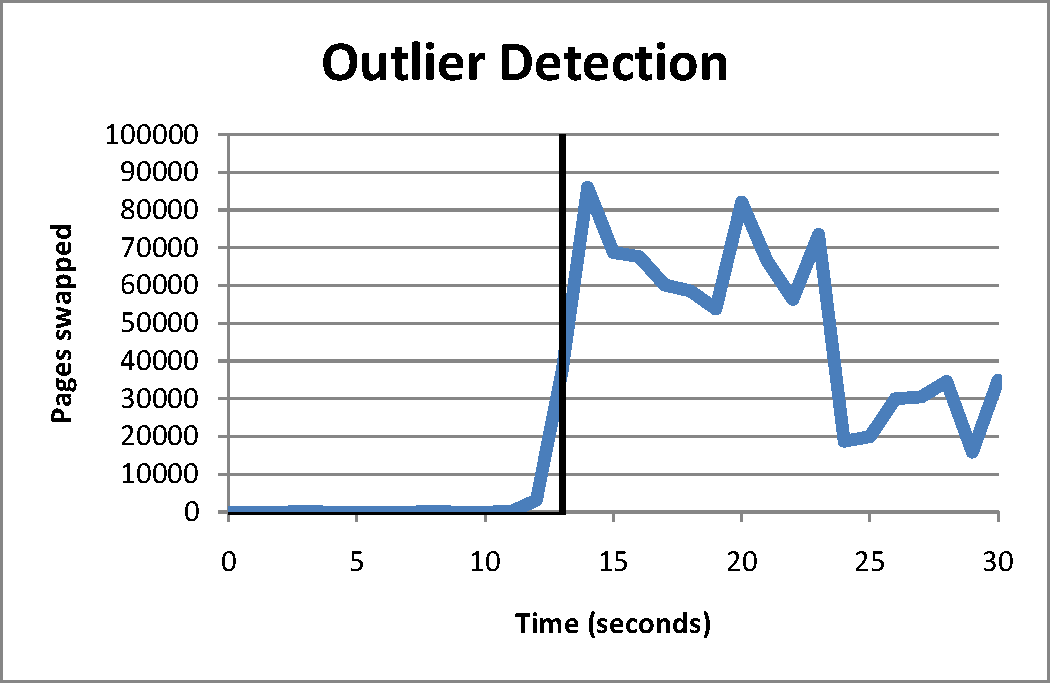
\includegraphics[scale=0.6]{figures/continue.pdf}
  \caption{Number of pages swapped over time on the thrashing host, as reported
    by \texttt{vmstat}.  The vertical line indicates the time at which the alert
    was sent by the monitoring system.}
\label{fig:outlier}
\end{figure}

To validate our prototype system monitoring tool, we constructed a
scenario in which one member of a MapReduce cluster begins thrashing
during the execution of a job. Our goal was to test how quickly our
monitoring system would detect this behavior. The basic mechanism is
similar to an alert system one of the authors implemented at an
Internet search company.

We used a simple load metric (a linear combination of CPU utilization,
paging, and swap activity). The continuous reduce function maintains
windows over samples of this metric: at regular intervals, it
compares the 20 second moving average of the load metric for each host
to the 120 second moving average of all the hosts in the cluster
{\em except} that host.  If the given host's load metric is more
than two standard deviations above the global average, it is
considered an outlier and a tentative alert is issued.  To dampen
false positives in ``bursty'' load scenarios, we do not issue an alert
until we have received 10 tentative alerts within a time window.

We deployed this system on an EC2 cluster consisting of 7 ``large''
nodes (large nodes were chosen because EC2 allocates an entire
physical host machine to them). We ran a wordcount job on the 5.5GB Wikipedia
data set, using 5 map tasks and 2 reduce tasks (1 task per host). After
the job had been running for about 10 seconds, we selected a node
running a task and launched a program that induced thrashing.

We report detection latency in Figure~\ref{fig:outlier}. The vertical bar
indicates the time at which the monitoring tool fired a (non-tentative)
alert. The thrashing host was detected very rapidly---notably faster than the
5-second {\TT}-{\JT} heartbeat cycle that is used to detect straggler tasks in
stock Hadoop. We envision using these alerts to do early detection of stragglers
within a MapReduce job: HOP could make scheduling decisions for a job by running
a secondary continuous monitoring query. Compared to out-of-band monitoring
tools, this economy of mechanism---reusing the MapReduce infrastructure for
reflective monitoring---has benefits in software maintenance and system
management.

\section{\BOOM-MR Port}
\label{ch:hop:sec:boom}

This chapter describes our port of the \BOOM-MR (Chapter~\ref{ch:boom}) to HOP.
Using \BOOM-MR, we developed alternative scheduling policies, written in
\OVERLOG, that made use of statistics provided by the monitoring system
described in Chapter~\ref{ch:hop:sec:monitor}.  In
Chapter~\ref{ch:hop:sec:jolport}, we describe the port of \JOL to the HOP \JT
scheduling component.  Chapter~\ref{ch:hop:sec:jolmonitor} describes the
interface between the monitoring system and \JOL, which enables the use of the
monitoring results in our declarative scheduling logic.  In
Chapter~\ref{ch:hop:sec:speculation}, we present an \OVERLOG rule that monitors
tasks for anomalous behavior~\cite{hopdemo}; spawning a backup/speculative task
when alerted to a potential issue.

\subsection{Scheduling HOP with \JOL}
\label{ch:hop:sec:jolport}

HOP is based on Hadoop 19.2, which defines an extensible interface to the \JT
scheduler component for alternative scheduler implementations.  This made the
port of \JOL to HOP trivial: the entire port consisted of $55$ lines of Java
glue code that implemented the \JOL harness, and \OVERLOG code that performed
the basic FIFO policy described in Chapter~\ref{ch:boom}.  We altered the job
relation (described in Table~\ref{ch:boom:tbl:hcatalog}) to include an
attribute for the job type: pipelining/blocking, online aggregation, or
continuous.  We also added three new scheduling rules (presented in
Figure~\ref{ch:hop:fig:schedmaps}) specific to online aggregation and
continuous jobs.

\subsubsection{\JOL Port}
\begin{figure*}
\ssp
\begin{minipage}{\linewidth}
\centering
\begin{verbatim}
public abstract class TaskScheduler implements Configurable {
   ...
   
  public abstract List<Task> 
  	assignTasks(TaskTrackerStatus taskTracker) throws IOException;
}
\end{verbatim}
\end{minipage}
\caption{Task scheduler interface. Not all methods shown.}
\label{ch:hop:fig:taskscheduler}
\end{figure*}


In Hadoop 19.2, the \JT makes use of an interface called the {\em
TaskScheduler} to implement alternative task scheduling policies.
Figure~\ref{ch:hop:fig:taskscheduler} shows a partial view of this interface,
which contains the method \ol{assignTasks} that is passed a \TT status object
and returns a list of tasks that should be scheduled.  This method is called by
the \JT during a {\em heartbeat} exchange with a \TT.

Our implementation of the \ol{assignTasks} method transforms the \TT status
object into a tuple that updates the \ol{taskTracker} relation in
Table~\ref{ch:boom:tbl:hcatalog}.  In response to this update, the scheduling
rules enter a fixpoint computation, during which it may assign task attempts to
the given \TT.  Any updates to the {\em schedule} relation (see rule \ol{s5} in
Figure~\ref{ch:boom:fig:schedule}) will trigger a (pre-registered) Java
listener that translates the update into a {\em Task} object, which the
\ol{assignTasks} method accumulates in a {\em List} object that is returned by
the \ol{assignTasks} method at the end of the fixpoint.

\subsubsection{Job submission interface}

The Hadoop {\JT} interface for submitting jobs had to be retrofitted to support
pipelining between jobs.  In regular Hadoop, jobs are submitted one at a time;
a job that consumes the output of one or more other jobs cannot be submitted
until the producer jobs have completed.  To support this, we modified the
Hadoop job submission interface to accept a list of jobs, where each job in the
list depends on the job before it.  The client interface traverses this list,
annotating each job with the identifier of the job that it depends on.  We then
added a new table to the declarative scheduler that captured inter-job
dependencies.  The job scheduling rules use this table to co-schedule jobs with
their dependencies, giving slot preference to ``upstream'' jobs over the
``downstream'' jobs they feed.  As we note in Chapter~\ref{ch:conclusion},
there are many interesting options for scheduling pipelines or even DAGs of
such jobs that we plan to investigate in future.


\subsubsection{Online aggregation and continuous job scheduling policies}

\begin{figure}
\ssp
\centering
\begin{lstlisting}
h1 unscheduledReduceTasks(JobId, a_count<TaskId>) :-
   job(JobId, JType, ...),
   task(JobId, TaskId, TType, Status, ...),
   JType == JobType.ONLINE, TType == TaskType.REDUCE,
   Status.state() != TaskState.RUNNING;

h2 canScheduleMaps(JobId) :-
   unscheduledReduceTasks(JobId, Count),
   Count == 0;

h3 canScheduleMaps(JobId) :-
   job(JobId, Type, ...),
   Type != JobType.ONLINE;
\end{lstlisting}
\caption{\label{ch:hop:fig:schedmaps} Counts the number of reduce tasks that are not running and 
only schedules map tasks from an online job when this count is zero.}
\end{figure}

Online aggregation and continuous jobs rely on a scheduling policy that ensures
the execution of the entire pipeline.  In the case of online aggregation, a
more complete pipeline provides more accurate estimates since unscheduled
partitions (i.e., groups) may contain important data.  For continuous jobs,
scheduling the entire pipeline is a requirement in order to avoid the memory
pressure in storing the (continuously arriving) data for an unscheduled
operator.  We enforced this constraint with by a policy that scheduled reduce
tasks before any map tasks in the same job (assuming sufficient slot capacity).

Figure~\ref{ch:hop:fig:schedmaps} shows three rules that together determine
when a job is allowed to schedule map tasks.  A separate admission controller
rule ensured that the number of reduce tasks for an online aggregation or
continuous job fit within the current cluster-wide slot capacity.  For each
job, rule \ol{h1} counts the number of reduce tasks not currently running.  If
the job type is ``online'' then rule \ol{h2} will add the fact that map tasks
can be scheduled when the number of non-running map tasks is equal to zero.
Rule \ol{h3} applies to the map tasks in all other job types; it simply removes
this scheduling constraints on those map tasks.  The \ol{canScheduleMaps}
predicate is included in the rule that determines the scheduling of map tasks
(e.g., rule \ol{s4} in Figure~\ref{ch:boom:fig:schedule}).

\section{Real-time monitoring with \JOL}
\label{ch:hop:sec:jolmonitor}

After porting \BOOM-MR to HOP, we started writing scheduler policies based on
the real-time monitoring information supplied by our monitoring job.  In order
to do this, we needed to import the results of our MapReduce monitoring job
into \JOL as relations.  Here, we further describe the MapReduce job that
continuously monitors HOP and its interface to \JOL.  We then present an alert
system that detects outlier measurements in map and reduce task execution
attempts.  We conclude our discussion with a new task speculation policy that
is based on our alert system.

\subsection{MapReduce monitoring job}

\begin{table}
\ssp
\centering
\begin{tabular}{|l|l|l|} \hline
\textit{Measure}    & \textit{Description}                 & \textit{Source} \\ \hline \hline
COMP\_EST        & Task estimated completion time  & \OVERLOG \\ \hline
USER\_CPU        & User CPU usage                   & /proc/stat, /proc/[pid]/stat \\ \hline
SYS\_CPU           & System CPU usage              & /proc/stat, /proc/[pid]/stat \\ \hline
RSS                       & Resident set memory size   & /proc/[pid]/stat   \\ \hline
VSIZE                    & Estimated completion time  & /proc/[pid]/stat  \\ \hline
WRITE\_BYTES   & Number of bytes written       & /proc/[pid]/io  \\ \hline
READ\_BYTES   & Number of bytes read           & /proc/[pid]/io \\ \hline
NET\_OUT           & Network output                      & /proc/net/dev \\ \hline
NET\_IN               & Network input                        & /proc/net/dev \\ \hline
SWAP\_OUT       & Swaps out                              & /proc/vmstat  \\ \hline
SWAP\_IN           &  Swaps in                               & /proc/vmstat \\ \hline
PAGE\_OUT       & Pages out                               & /proc/vmstat \\ \hline
PAGE\_IN           & Pages in                                 & /proc/vmstat \\ \hline
\end{tabular}
\caption{HOP monitoring measurements.}
\label{ch:hop:tbl:measure}
\end{table}

The MapReduce job that monitors HOP is scheduled during the system bootstrap.
The job executes a single map task on each \TT in the cluster and some
number (based on the size of the cluster) of reduce tasks that group machine
and rack level statistics.  For example, we could schedule a single reduce task
per rack that aggregates the statistics gathered on that rack.

Table~\ref{ch:hop:tbl:measure} lists the measurements that we collected.  The
measurement name is given in the first column, followed by a measurement
description.  The last column identifies the location under \ol{/proc} where
the measurement was taken.  Process level measurements reside under
\ol{/proc/[pid]/}, where \ol{[pid]} represents the process identifier.  All
other measurements outside of \ol{/proc/[pid]/} refer to machine level
measurements with the exception of the estimated completion time, which is
derived from task level statistics in the \JT.

A map task gathers measurements by periodically reading the source location
(last column in Table~\ref{ch:hop:tbl:measure}) from the local file system.
For each measurement, the map task outputs a record \ol{<host name, time stamp,
pid, measurement name, measurement value>}.  For machine statistics, the map
task will set the $PID$ field to {\underline 0} e.g.,
\ol{<boom.cs.berkeley.edu, 12348234, {\underline 0}, NET\_OUT, 101>}.  The
record key for all map outputs is the identifier of the rack to which the
machine belongs.  If the cluster does not contain rack-level information then
the host name is used instead.  This ensures that a single reduce task will see
all measurements from a given rack or machine boundary.

\subsection{Monitoring with \OVERLOG}
\label{ch:hop:sec:omonitor}

\begin{table}
\ssp
\centering
\begin{tabular}{|l|l|l|} \hline
\textit{Name}    & \textit{Description} & \textit{Relevant attributes} \\ \hline\hline
machineStat    & Machine statistics   & \underline{Host}, \underline{Measure}, TimeStamp, Value \\ \hline
proccessStat   & Process statistics    & \underline{TaskId}, \underline{Pid}, \underline{Measure}, TimeStamp, Value \\ \hline
jobStat              & Job statistics            & \underline{JobId}, \underline{TaskType}, \underline{Measure}, StatContainer \\ \hline
taskStat            & Task statistics          & \underline{JobId}, \underline{TaskId}, \underline{Measure}, TaskType, Value \\ \hline
alert                   & Outlier task alerts   & \underline{TaskId}, \underline{TimeStamp}, \underline{Measure}, \\
                           &                                   & Description, Severity \\ \hline
\end{tabular}
\caption{\JOL monitoring relations.}
\label{ch:hop:tbl:monitorCatalog}
\end{table}

The output of the monitoring job is sent directly --- reduce tasks open a
back-channel TCP-socket --- to the \JOL instance running on the \JT.  The
receiver code translates the data packets into \JOL tuples, and inserts them
into monitoring relations defined in Table~\ref{ch:hop:tbl:monitorCatalog}.
The \ol{machineStat} and \ol{processStat} tables are populated by the data
packets received from the monitoring jobs.  The \ol{jobStat} and \ol{taskStat}
tables maintain statistics for jobs and tasks, respectively, and are derived by
\OVERLOG rules (Figures~\ref{ch:hop:fig:taskstat}
and~\ref{ch:hop:fig:jobstat}).  The \ol{alert} table contains outlier task
measurements, which depending on the severity can result in corrective action
e.g., execute a speculative task (Chapter~\ref{ch:hop:sec:speculation}).

\begin{figure}
\ssp
\centering
\begin{lstlisting}
/* Correlate process measurements to the actual map/reduce task */
ts1 taskStat(TaskId.getJobID(), TaskId, Measure, Type, TimeStamp, 
             Value) :-
    taskAttempt(TaskId, ... , TaskState.RUNNING, Pid),
    processStat(Host, Pid, Measure, TimeStamp, Value),
    Type := TaskId.isMap() ? TaskType.MAP : TaskType.REDUCE;
        
/* Compute the estimated completion time based on the task rate 
   of progress */
ts2 taskStat(JobId, TaskId, COMP_EST, TaskType, TimeStamp, CompEst) :-
    taskAttempt(TaskId, ... , Progress, ProgressRate, TaskState.RUNNING, 
                Pid),
    JobId := TaskId.getJobID(),
    Type := TaskId.isMap() ? TaskType.MAP : TaskType.REDUCE,
    CompEst := ProgressRate == 0 ? infinity : 
               (1f - Progress) / ProgressRate,
    TimeStamp := java.lang.System.currentTimeMillis();
\end{lstlisting}
\caption{\label{ch:hop:fig:taskstat} Rules for maintaining the \ol{taskStat} table.}
\end{figure}

Figure~\ref{ch:hop:fig:taskstat} contains two rules that together maintain the
\ol{taskStat} table.  The \ol{taskAttempt} table was extended to include the
task process identifier ($Pid$), which is supplied by the \TT executing the
task attempt.  The process identifier allows us to correlate a task in the
\ol{taskAttempt} table with process level measurements in the \ol{processStat}
table, as shown by rule \ol{ts1}.  A task's estimated completion time is based
on its current progress and progress rate: change in progress computed over \TT
heartbeat intervals.  Using the current progress and progress rate, rule
\ol{ts2} computes a rough estimate on the remaining time it will take for the
task to complete, which we have denoted as a COMP\_EST measurement --- stored
in the \ol{taskStat} table.

\begin{figure}
\ssp
\centering
\begin{lstlisting}
js1 taskStatList(JobId, TaskType, Measure, a_list<Value>) :-
    taskStat(JobId, TaskId, Measure, TaskType, TimeStamp, Value);

        
js2 jobStat(JobId, TaskType, Measure, Statistics) :-
    taskStatList(JobId, TaskType, Measure, TaskStatList),
    Statistics := new StatContainer(TaskStatList);
\end{lstlisting}
\caption{\label{ch:hop:fig:jobstat} Rules for maintaining the \ol{jobStat} relation.}
\end{figure}

Figure~\ref{ch:hop:fig:jobstat} contains the rules for maintaining the
\ol{jobStat} table.  The \ol{taskStatList} table, maintained by rule \ol{js1},
provides a list of measurement values for each job identifier, task type, and
measurement name.  The \ol{jobStat} table groups measurement values belonging
to the same job, task type, and measurement name.  A special Java object called
{\em StatContainer} is used to store each group of measurements.  The {\em
StatContainer} class defines methods for computing various metrics (e.g., mean,
median, stddev, etc.) from its list of measurement values.  Rule \ol{js2}
maintains the \ol{jobStat} table by initializing a {\em StatContainer} object
for each group of aggregated measurement values.


\subsection{Task alerts} 

\begin{figure}
\ssp
\centering
\begin{lstlisting}
a1 alert (TaskId, TimeStamp, Measure, Desc, Severity) :-
   taskStat(JobId, TaskId, Measure, TaskType, TimeStamp, TaskStat),
   jobStat(JobId, TaskType, Measure, JobStat),
   JobStat.outlier(Measure, TaskStat) == true,
   Desc := JobStat.description(Measure, TaskStat),
   Severity := JobStat.severity(Measure, TaskStat),
   TimeStamp := java.lang.System.currentTimeMillis();
\end{lstlisting}
\caption{\label{ch:hop:fig:outlier} Rule for detecting outlier tasks. }
\end{figure}

Figure~\ref{ch:hop:fig:outlier} contains a single rule that detects outlier
task by correlating the task measurement with information in the \ol{jobStat}
table.  We compare the measurements from tasks that belong to the same category
--- job and task type (map or reduce).  The $JobStat$ variable references a {\em
StatContainer} object for a given category, and it is used to determine if a
task belonging to that category is an outlier based on some metric e.g., $k$
deviations from the mean.  The $JobStat$ variable is also used to provide a
description and severity of outlier measurement.

\subsection{Alert based speculation policy} 
\label{ch:hop:sec:speculation}

\begin{figure}
\ssp
\centering
\begin{lstlisting}

s1 mostRecentCriticalAlert(TaskId, Measure, a_min<AlertTime>) :-
   alert(TaskId, AlertTime, Measure, Desc, Severity),
   Severity.contains(``critical'');  /* The alert is critical */

s2 schedule(Tracker, list<TaskId, MapSlots>) :-
   heartbeat(Tracker, TrackerStatus, MapSlots, _),
   MapSlots > 0,
   mostRecentCriticalAlert(TaskId, Measure, AlertTime)

   /* Ensure the alert is not too old (alert time < 10 seconds ago). */
   (java.lang.System.currentTimeMillis() - AlertTime) < 10000,

   /* The task's estimated time to completion is very high relative
      to equivalent tasks. */
   taskStat(JobId, TaskId, COMP_EST, TaskType, TimeStamp, TaskStat),
   jobStat(JobId, TaskType, COMP_EST, JobStat),
   TaskStat < JobStat.percentile(0.25),

   /* Schedule backup map task if host has split AND 
      no backup task has yet been scheduled */
   task(JobId, TaskId, ..., Splits, ...), TaskId.isMap(),
   taskAttemptCount(TaskId, Count), Count == 1,
   InputSplits.contains(TrackerStatus.getHost());
\end{lstlisting}
\caption{\label{ch:hop:fig:speculation} 
Rule for map task speculation based on alert system data. Reduce task 
speculation rule is similar (we do no consider splits) and therefore omitted. }
\end{figure}    
   
Figure~\ref{ch:hop:fig:speculation} contains a rule that reschedules map tasks
with any ``critical'' alerts that occurred recently; rule~\ol{s1} defines the
\ol{mostRecentCriticalAlert} relation.  Rule~\ol{s2} is evaluated at the \JT
whenever a {\em heartbeat} exchange occurs with some \TT.  The \ol{heartbeat}
predicate includes the name of the \TT, its status, and its spare map slot
capacity, which the rule ensures is greater than zero.  The rule joins the
\ol{heartbeat} with all critical alerts in the \ol{mostRecentCriticalAlert}
relation.  As an added precaution, we subsequently check that the alerted
task's estimated completion (\ol{COMP\_EST}) time is high relative to other
tasks in its category.  Finally, we ensure that the task has not already been
rescheduled and that the \TT contains the maps input data.


\subsection{Evaluation}

\begin{figure*}[ht]
\ssp
  \centering
  \subfloat[][Hadoop 19.2 task speculation policy]{\label{fig:spec-hadoop}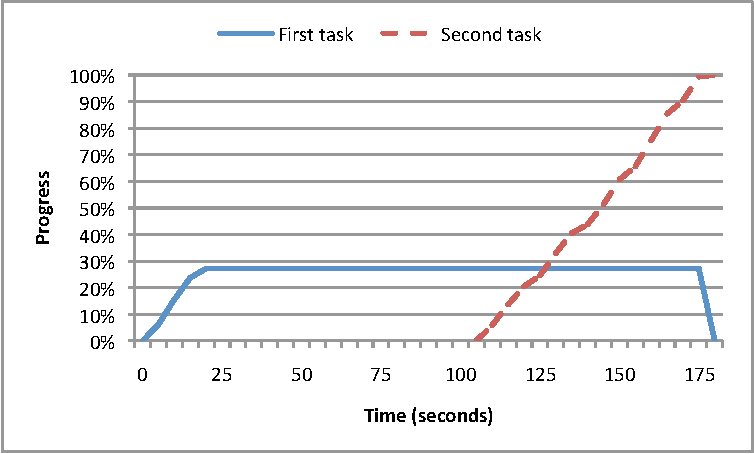
\includegraphics[width=0.48\linewidth]{figures/taskSpecPolicy_vanilla}}
  \subfloat[][HOP alert based task speculation policy]{\label{fig:spec-hop}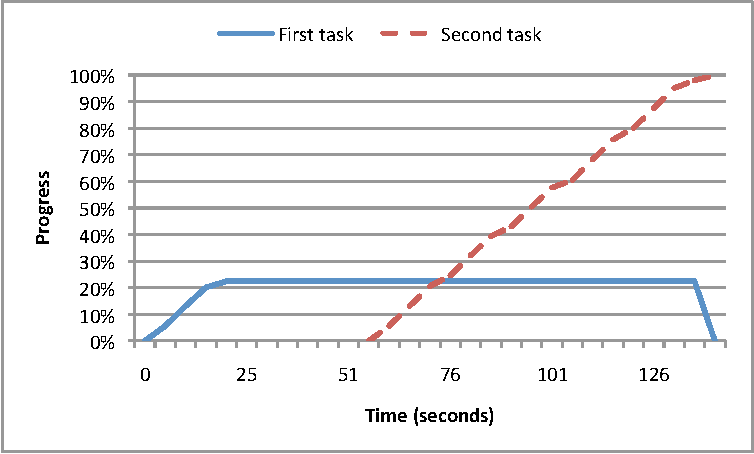
\includegraphics[width=0.48\linewidth]{figures/taskSpecPolicy_hop}}
  \caption{Compares speculation policies by plotting the starting point and progress of the faulty task (first task) and speculative task (second task).}
\label{fig:taskSpecPolicy}
\end{figure*}

We compared our alert based speculation policy with the speculation policy
implemented in unmodified Hadoop 19.2.  Our experiment executed a wordcount job
that contained a single faulty map task that would execute normally for a
minute before stalling out by sleeping for one second intervals between map
function invocations.  The input to the wordcount was 10GB of randomly
generated words, yielding 20 map tasks total.  We executed this job on a 20
node EC2 cluster and compared the time it took to initiate a speculative task
using our policy to the policy in unmodified Hadoop.

Figure~\ref{fig:taskSpecPolicy} shows the result of this experiment by plotting
the launch time and progress of the original (first) task and the backup
(second) task.  HOP's alert based speculation policy is able to detect the
faulty map task and execute a backup task in half the time of unmodified
Hadoop.  In unmodified Hadoop, a task is speculated based on its rate of
progress (relative to other tasks in its category).  We are able to further
extend this policy by including machine and process level statistics as further
evidence to speculate.  Indeed, our choice to speculate was not only based on a
high estimated time to completion but also a critically low ``user CPU'' value
and a critically low I/O activity.

The astute reader will notice however that the rate of progress for the second
task in HOP is less than that of unmodified Hadoop.  The reason for this is
that our monitoring jobs do add some extra load to the cluster.  Nevertheless,
in this instance, the overall job response time was slightly less (a few
seconds) in HOP due to the faster turn around time in our speculation policy.


\section{Related Work}
\label{ch:hop:sec:relwork}

This work relates to literature on parallel dataflow frameworks, online
aggregation, and continuous query processing.

\subsection{Parallel Dataflow}

Dean and Ghemawat's paper on Google's MapReduce~\cite{mapreduce-osdi} has
become a standard reference, and forms the basis of the open-source Hadoop
implementation.  The Google MapReduce design targets very large clusters where
the probability of worker failure or slowdown is high.  This led to their
elegant checkpoint/restart approach to fault-tolerance, and their lack of
pipelining.  Our work extends the Google design to accommodate pipelining
without significant modification to their core programming model or fault
tolerance mechanisms.

{\em Dryad}~\cite{dryad07} is a data-parallel programming model and runtime
that is often compared to MapReduce, supporting a more general model of acyclic
dataflow graphs.  Like MapReduce, Dryad puts disk materialization steps between
dataflow stages by default, breaking pipelines.  The Dryad paper describes
support for optionally ``encapsulating'' multiple asynchronous stages into a
single process so they can pipeline, but this requires a more complicated
programming interface.

It has been noted that parallel database systems have long provided partitioned
dataflow frameworks~\cite{pavlo09}, and recent commercial databases have begun
to offer MapReduce programming models on top of those
frameworks~\cite{aster,greenplum}.  Most parallel database systems can provide
pipelined execution akin to our work here, but they use a more tightly coupled
iterator and {\em Exchange} model that keeps producers and consumers
rate-matched via queues, spreading the work of each dataflow stage across all
nodes in the cluster~\cite{exchange}.  This provides less scheduling
flexibility than MapReduce and typically offers no tolerance to mid-query
worker faults.  Yang et al.\ recently proposed a scheme to add support for
mid-query fault-tolerance to traditional parallel databases, using a
middleware-based approach that shares some similarities with
MapReduce~\cite{osprey-icde}.

Logothetis and Yocum describe a MapReduce interface over a continuous query
system called {\em Mortar} that is similar in some ways to our
work~\cite{logoyocum08}.  Like HOP, their mappers push data to reducers in a
pipelined fashion.  They focus on specific issues in efficient stream query
processing, including minimization of work for aggregates in overlapping
windows via special reducer APIs.  They are not built on Hadoop, and explicitly
sidestep issues in fault-tolerance.

{\em Hadoop Streaming} is part of the Hadoop distribution, and allows map and
reduce functions to be expressed as UNIX shell command lines.  It does not
stream data through map and reduce phases in a pipelined fashion.

\subsection{Online Aggregation}

Online aggregation was originally proposed in the context of simple
single-table SQL queries involving ``Group By'' aggregations, a workload quite
similar to MapReduce~\cite{onlineagg}.  The focus of the initial work was on
providing not only ``early returns'' to these SQL queries, but also
statistically robust estimators and confidence interval metrics for the final
result based on random sampling.  These statistical matters do not generalize
to arbitrary MapReduce jobs, though our framework can support those that have
been developed.  Subsequently, online aggregation was extended to handle join
queries (via the {\em Ripple Join} method), and the {\em CONTROL} project
generalized the idea of online query processing to provide interactivity for
data cleaning, data mining, and data visualization tasks~\cite{ieeecontrol}.
That work was targeted at single-processor systems.  Luo et al.\ developed a
partitioned-parallel variant of Ripple Join, without statistical guarantees on
approximate answers~\cite{luo-ripple}.

In recent years, this topic has seen renewed interest, starting with Jermaine
et al.'s work on the {\em DBO} system~\cite{dbo}.  That effort includes more
disk-conscious online join algorithms, as well as techniques for maintaining
randomly-shuffled files to remove any potential for statistical bias in
scans~\cite{jermaine-shuffle}.  Wu et al.\ describe a system for peer-to-peer
online aggregation in a distributed hash table context~\cite{wu-vldb09}.  The
open programmability and fault-tolerance of MapReduce are not addressed
significantly in prior work on online aggregation.

An alternative to online aggregation combines precomputation with sampling,
storing fixed samples and summaries to provide small storage footprints and
interactive performance~\cite{gibbons98new}.  An advantage of these techniques
is that they are compatible with both pipelining and blocking models of
MapReduce.  The downside of these techniques is that they do not allow users to
choose the query stopping points or time/accuracy trade-offs
dynamically~\cite{ieeecontrol}.

\subsection{Continuous Queries}

In the last decade there was a great deal of work in the database research
community on the topic of continuous queries over data streams, including
systems such as Borealis~\cite{borealis}, STREAM~\cite{stream}, and
Telegraph~\cite{tcq-cidr}.  Of these, Borealis and Telegraph~\cite{flux-ft}
studied fault-tolerance and load balancing across machines.  In the Borealis
context this was done for pipelined dataflows, but without partitioned
parallelism: each stage (``operator'') of the pipeline runs serially on a
different machine in the wide area, and fault-tolerance deals with failures of
entire operators~\cite{borealisFT}.  SBON~\cite{sbon} is an overlay network
that can be integrated with Borealis, which handles ``operator placement''
optimizations for these wide-area pipelined dataflows.

Telegraph's {\em FLuX} operator~\cite{flux-ft,flux-lb} is the only work to our
knowledge that addresses mid-stream fault-tolerance for dataflows that are both
pipelined and partitioned in the style of HOP\@.  FLuX (``Fault-tolerant,
Load-balanced eXchange'') is a dataflow operator that encapsulates the
shuffling done between stages such as map and reduce.  It provides
load-balancing interfaces that can migrate operator state (e.g., reducer state)
between nodes, while handling scheduling policy and changes to data-routing
policies~\cite{flux-lb}.  For fault-tolerance, FLuX develops a solution based
on process pairs~\cite{flux-ft}, which work redundantly to ensure that operator
state is always being maintained live on multiple nodes.  This removes any
burden on the continuous query programmer of the sort we describe in
Chapter~\ref{ch:hop:sec:continuous}.  On the other hand, the FLuX protocol is
far more complex and resource-intensive than our pipelined adaptation of
Google's checkpoint/restart tolerance model.

\section{Summary}

In this chapter, we extended the batch-oriented execution model of MapReduce to
support pipelining between operators.  This enables a new suite of MapReduce
jobs that are able to perform online aggregation and continuous like queries.
Unlike much of the work on online aggregation, we do not focus here on
statistical guarantees because of the flexibility of the MapReduce programming
model.  These guarantees are crafted for specific SQL aggregates like SUMs,
COUNTs, and AVERAGEs, and modified to account for processing techniques like
the join algorithms used.  The focus of our work here is architectural: to
provide ``early returns'' interactions within the powerful scalability and
fault-tolerance facilities of MapReduce frameworks.  The statistical guarantees
from the literature only apply to SQL-style reduce functions; statistical
guarantees for other online reducers would need to be developed in a
case-by-case basis.  We expect that in many cases users will settle for simply
observing changes in the output of a job over time, and make their own
decisions about whether early returns are sufficient.

We leveraged our ability to run continuous MapReduce jobs in HOP by developing
a monitoring framework that provides near real-time machine and process level
statistics.  Our monitoring framework enabled new scheduling opportunities that
are based on such statistics.  Porting the declarative scheduler to HOP allowed
us to quickly prototype alternative policies in \OVERLOG where, in many cases,
adding new scheduling constraints translated into adding/removing a few rule
predicates.



